\documentclass[11pt,oneside,a4paper]{article}
\usepackage[top=2cm, left=2cm, right=2cm, bottom=2cm]{geometry}
\usepackage{color}
\usepackage{pdfpages}
\usepackage{graphicx}
\usepackage{float}
\usepackage{listings}
\usepackage[british]{babel}
\usepackage{bold-extra}
\usepackage{array}
\usepackage{longtable}
\usepackage{caption}
\usepackage[pdfborder={0 0 0}]{hyperref}
\usepackage{amsmath}

\emergencystretch=3cm

\setcounter{secnumdepth}{4}
\setcounter{tocdepth}{4}

\lstset{
  breaklines=true,
  breakindent=0pt,
  basicstyle=\small\ttfamily,
  language=C++
}

\begin{document}
\title{QKD-Simulate - Documentation}
\author{Program Authors: \\
  \\
  Oliver Maurhart \\
  Mario Kahn \\
  Philipp Grabenweger \\
  \\
  Documentation Author: \\
  \\
  Philipp Grabenweger
}
\date{September 2013}
\maketitle

\newpage

\begin{abstract}
This document describes the design principles, program internals and underlying physical and mathematical models of the QKD-Simulate program. Its purpose is to provide an insight into the concepts of program design and enable the reader to change or enhance the program's functionality.
\end{abstract}

\newpage
\tableofcontents

\listoffigures

\listoftables

\newpage
\section{Overview}
\label{sec:overview}

QKD-Simulate is a program written in C++11 with a GUI based on the Qt library that simulates key generation according to the BB84 quantum key distribution scheme. The basic components of the system simulated by this program are shown in Figure \ref{fig:quantum_channel}.

\begin{figure}[h]
\centering
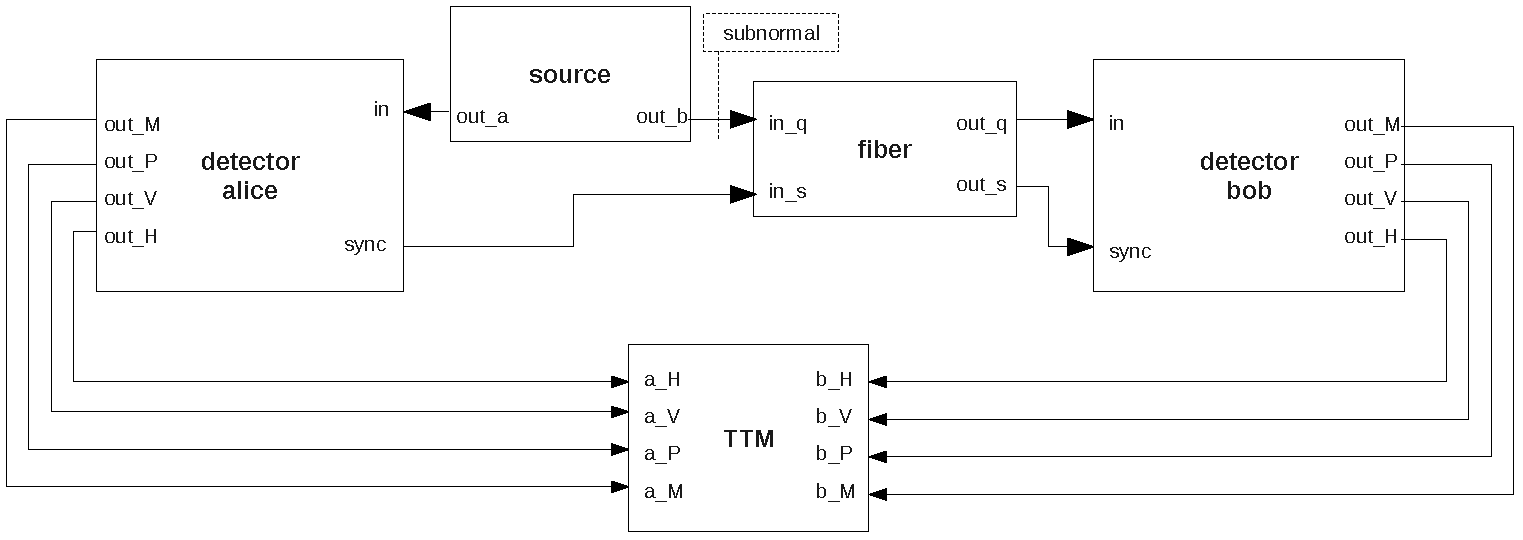
\includegraphics[scale=0.65]{drawings/channel.pdf}
\caption{The quantum key distribution system as modelled by the \texttt{channel} class}
\label{fig:quantum_channel}
\end{figure}

Actually, the components shown as rectangles with solid lines in this figure are instances of C++ classes that are defined in \texttt{.cpp} and \texttt{.h} files in the \texttt{channel} subdirectory of the \texttt{qkd-simulate} directory. Concretely, \textbf{source} is an instance of the \texttt{source} class defined in \texttt{source.h} and \texttt{source.cpp}, \textbf{fiber} is an instance of the \texttt{fiber} class defined in \texttt{fiber.h} and \texttt{fiber.cpp}, \textbf{TTM} is an instance of the \texttt{ttm} class defined in \texttt{ttm.h} and \texttt{ttm.cpp}, and \textbf{detector alice} and \textbf{detector bob} are two instances of the \texttt{detector} class defined in \texttt{detector.h} and \texttt{detector.cpp}, where a flag stored as a class member with name \texttt{m\_bAlice} of type \texttt{bool} is set to \texttt{true} for Alice's side and to \texttt{false} for Bob's side by a parameter named \texttt{bAlice} passed to the constructor at class instantiation. All of these class instances 
are contained in an instance of the \texttt{channel} class defined in \texttt{channel.h} and \texttt{channel.cpp} that manages the whole quantum key distribution simulation.
\\
\\
The physical process that should be simulated by this system is the following: The EPR (Einstein-Podolsky-Rosen) source creates pairs of entangled photons with a specific photon rate. For each created pair, one of the photons travels to the detector at Alice's side, the other one is transmitted over an optical fiber and travels to the detector at Bob's side. At first, the polarisation of the photon received by Alice's detector is measured in either the H/V (horizontal/vertical) or P/M (plus/minus) base (one of the two bases is selected randomly with equal probability\footnote{Changing this to unequal probabilities requires adaption of the \texttt{detector\_optics} class defined in \texttt{channel/detector/detector\_optics.h} and \texttt{channel/detector/detector\_optics.cpp}}) which causes a collapse of the entangled quantum state and determines the polarisation of the second photon (travelling to Bob's detector) which must be orthogonal to the polarisation state measured for the first photon by Alice's 
detector. Then, after some transmission delay time, the second photon is received by Bob's detector and its polarisation is measured in again either the H/V or the P/M basis chosen randomly. Alice's as well as Bob's detector contain four single-photon detection elements, one for each of the four possible photon polarisations.
\\
\\
What happens next depends on the system configuration:

\begin{itemize}

\item In the \textit{free running mode}, the single-photon detectors at Alice's and Bob's sides are enabled permanently, and for all received photons at Alice's or Bob's sides the TTM (Time Tagging Module) records the detection time and measured polarisation. In Figure \ref{fig:quantum_channel} only one TTM object is shown because in the C++ program, the \texttt{ttm} class is only instantiated once for simplicity, but in reality both Alice and Bob have their own TTM module.

\item In the \textit{sync mode} (for which also exist several variants that will be described later) the photon received by Alice's detector causes the generation of a sync pulse that is also transmitted over the fiber, but at another wavelength using WDM (wavelength-division multiplexing). Only when Bob's detector receives the sync pulse, it enables its single-photon detectors for some time so that they are ready to receive the second photon, which comes to Bob's detector a bit later than the sync pulse because it also travels through a delay fiber (not shown in Figure \ref{fig:quantum_channel}). The electrical pulses coming out of the single-photon detectors at Alice's and Bob's sides during some time window are then used for generating a binary string (4 bits each time a sync pulse is sent/received) that is stored in a buffer.

\end{itemize}

\newpage
\section{Concepts of Program Design}
\label{sec:concepts}

In this section, the basic principles and concepts of the design of the QKD simulator will be described. It will be explained how components that are part of the simulation system can interact, which requirements they have to fulfil and which behaviour is expected from them. 

\subsection{Object-Oriented Design and Event-Oriented Simulation}

The physical system as described in section~\ref{sec:overview} is modelled and simulated with objects that are instances of C++ classes, which are interacting by sending events to each other. All classes that define the structure of components which are interacting in the simulation by sending and receiving events are derived from the base class \texttt{channel\_event\_handler} that defines basic functionality and interfaces necessary for event handling. 

Objects which are in the same level of containment hierarchy do not communicate directly, however, but only send events either to one of the objects it contains (further denoted as child event handlers), to themselves, or to the object containing them (further denoted as parent event handler). The parent event handler is responsible for establishing the connectivity between its child event handlers by forwarding those events that its child event handlers are sending to it, if necessary. 

For example, if the \textbf{source} in Figure \ref{fig:quantum_channel} is generating a new photon pair, it sends an event to its parent event handler which is the \textbf{channel}, which in turn forwards the event to \textbf{detector alice} and to \textbf{fiber} because these event handlers are connected to the \textbf{source}. This concept that components only send events to their parents or childs or to themselves, although it might seem restrictive, provides the advantage of flexibility when changing the system configuration and allows components to be instantiated multiple times without causing name conflicts and without the necessity to change their implementation.

\subsection{Management of the Simulation and Event Dispatch}
\label{subsec:concepts_events}

A central role in the simulation plays one instance of the class \texttt{channel\_event\_manager} which is owned by the \texttt{channel} object. All event handlers on their initialisation obtain a pointer to the \texttt{channel\_event\_manager} object so that they can access it. Also they call the \texttt{add\_event\_handler} function of the \texttt{channel\_event\_manager} to register themselves as event handlers participating in the simulation. The \texttt{channel\_event\_manager} provides the \texttt{add\_event} function that allows to insert a new event into an event priority queue which the \texttt{channel\_event\_manager} internally keeps. An event is stored as a class named \texttt{event} which is defined as shown in Listing \ref{lst:event}.

\begin{lstlisting}[caption={Definition of the \texttt{event} class}, captionpos=b, label={lst:event}]
class event {

    uint64_t nId;
    priority ePriority;
    type eType;
    channel_event_handler * cDestination;
    channel_event_handler * cSource;
    int64_t nTime;
    
    struct {
        
        uint64_t m_nPhotonPairId;
        photon_state m_ePhotonState;
        int64_t m_nDetectTime;
        bool m_bAlice;
        bool m_bDown;
        
    } cData;
};
\end{lstlisting}

The meaning of the structure members is the following:

\begin{itemize}

\item \texttt{m\_nTime} defines the time when the event should occur. It is measured in units of the \texttt{RESOLUTION} constant defined in the \texttt{ttm} class which is defined to be 82.3~ps, and the time is stored as signed 64-bit integer, so it is discretised to a time raster with a resolution of \texttt{ttm::RESOLUTION}.

\item \texttt{m\_ePriority} defines the event priority. It is one of the enumeration constants defined in the \texttt{channel\_event\_priority} enumeration type as shown in Listing \ref{lst:event_priority}. The highest priority is the first one, and the lowest the last one defined. Event priorities are required when several events occur at the same time to determine the order of event dispatch. In the case that multiple events are set to occur at the same time, the events are handled in the order of their priorities, with the event having the highest priority being handled first. For events that are set to the same time and that also have the same priority the order of their dispatch is not determined.

\item \texttt{m\_eType} describes the type of event, it must be one of the enumeration constants defined in the \texttt{channel\_event\_type} enumeration type in \texttt{event.h} (see Listing \ref{lst:event_type}).

\item \texttt{m\_cDestination} is the address of the channel event handler that should receive the event.

\item \texttt{m\_cSource} is the address of the channel event handler that sent the event.

\item \texttt{m\_cData} is a structure variable containing additional information required for specific events.

\end{itemize}

\begin{lstlisting}[caption={Definition of the \texttt{event\_priority} enumeration type}, captionpos=b, label={lst:event_priority}]
    enum priority : uint8_t {
        
        SYSTEM,
        SUPERHIGH,
        HIGH,
        NORMAL,
        SUBNORMAL,
        LOW
    };
\end{lstlisting}

\begin{lstlisting}[caption={Definition of the \texttt{channel\_event\_type} enumeration type}, captionpos=b, label={lst:event_type}]
    enum type : uint8_t {
        DARK_COUNT,
        DETECT,
        DETECTOR_PULSE,
        DISABLE,
        DOWN_END,
        ENABLE,
        INIT,
        PHOTON,
        PULSE,
        STOP,
        SYNC_PULSE,
        SYNC_PULSE_BAD,
        WINDOW_END,
        WINDOW_END_BAD,
        WINDOW_START
    };
\end{lstlisting}

All channel event handlers provide the \texttt{handle} function that receives an event structure as parameter (passed by reference) which describes the event that should be handled. The \texttt{channel\_event\_manager} has a member variable named \texttt{m\_nTime} that stores the current simulation time. When a simulation is run, the following steps are performed:

\begin{itemize}

\item The \texttt{channel\_event\_manager} clears its event priority queue and initialises its \texttt{m\_nTime} variable with zero.

\item The \texttt{channel\_event\_manager} sends events with \texttt{m\_eType} set to \texttt{channel\_event\_type::init} to all registered event handlers.

\item As long as the \texttt{channel\_event\_manager}'s event priority queue is not empty and not some stop criterion is fulfilled, the \texttt{channel\_event\_manager} repeats the following steps:

\begin{itemize}

\item The \texttt{channel\_event\_manager} takes the next event that should be processed (depending on the \texttt{m\_nTime} and \texttt{m\_ePriority} members of all events in the queue) out of its event priority queue. Let this event further be denoted by  \texttt{ev}.

\item \texttt{channel\_event\_manager.m\_nTime} is set to \texttt{ev.m\_nTime}.

\item The \texttt{handle} function of the channel event handler addressed by \texttt{ev.m\_cDestination} is called with \texttt{ev} being passed as parameter.

\end{itemize}

\item The \texttt{channel\_event\_manager} sends events with \texttt{m\_eType} set to \texttt{channel\_event\_type::stop} to all registered event handlers.

\end{itemize}

By following the procedure described above it is ensured that all generated events are processed in correct chronological order, provided that only causal event generation is allowed, which means that never an event may be generated that should occur at a time earlier than the current simulation time. To avoid hang-ups or stack overflows, a \texttt{channel\_event\_handler} should never call the \texttt{handle} function of another \texttt{channel\_event\_handler} directly, but should always only use the \texttt{channel\_event\_manager}'s \texttt{add\_event} function to generate new events that can eventually address a specific \texttt{channel\_event\_handler} that should receive the event (possibly after some forwarding).

\subsection{Management of Photon and Photon Pair Generation and Destruction}
\label{subsec:concepts_photons}

While the simulation is running, usually a large number of photons and photon pairs are generated by photon sources. Data structures are required to describe the properties like polarisation and entanglement of photons. Additionally, for pairs of entangled photons it is necessary to have a possibility to uniquely identify the two photons which are entangled, because measurement of the polarisation of one of the entangled photons instantaneously determines the polarisation state that will be measured for the other photon. For this purpose, the \texttt{photon\_state} enumeration type and the \texttt{photon\_pair} structure as shown in Listing \ref{lst:photon_pair} have been defined in \texttt{photon\_pair.h}.

\begin{lstlisting}[caption={Definition of the \texttt{photon\_state} enumeration type and the \texttt{photon\_pair} structure}, captionpos=b, label={lst:photon_pair}]
enum photon\_state : uint8_t {
    
    NONPOLARIZED,
    ENTANGLED,
    HORIZONTAL,
    VERTICAL,
    PLUS,
    MINUS,
    ABSORBED
};

struct photon_pair {
    
    photon_state eStateA;
    photon_state eStateB;
    double nEntanglementError;
};
\end{lstlisting}

The \texttt{photon\_pair} structure is used to describe single photons as well as pairs of entangled photons. The members of the structure have the following meaning:

\begin{itemize}

\item \texttt{eStateA} is the state of the photon travelling to Alice. It must be set to one of the enumeration constants defined in \texttt{photon\_state}.

\item \texttt{eStateB} is the state of the photon travelling to Bob. It must be set to one of the enumeration constants defined in \texttt{photon\_state}.

\item \texttt{nEntanglementError} is a probability value (must be between 0 and 1) only valid for a pair of entangled photons. It describes the probability of measuring the same instead of orthogonal polarisation for the two entangled photons when measured in the same base (either H/V or P/M) at both Alice's and Bob's side. If the second photon is measured in a different base than the first photon, the \texttt{entanglement\_error} value does not have any effect (both possible polarisation measurement results for the second photon still are equally probable). This means that the \texttt{entanglement\_error} property only models an unbiased statistical error.

\end{itemize}

Setting \texttt{eStateA} or \texttt{eStateB} to \texttt{photon\_state::ABSORBED} means either that the photon has never been created (because only a single photon should be described) or it is not existing anymore because it has been absorbed (due to transmission loss, measurement, etc.). The enumeration constant \texttt{photon\_state::ENTANGLED} has a special role and may only be used if both \texttt{eStateA} and \texttt{eStateB} are set to it. It describes a pair of entangled photons. The \texttt{photon\_state::NONPOLARIZED} state can be used to describe photons whose polarisation is not known and statistically distributed over all possibilities with equal probability. The other enumeration constants defined in \texttt{photon\_state} describe specific polarisation states of the H/V and P/M bases.

Because the allocation of heap memory each time a \texttt{photon\_pair} structure is needed would be inefficient in consideration of the runtime and therefore slow down the simulation, a \texttt{photon\_pair\_manager} class has been defined. The \texttt{channel} object keeps an instance of this class (which is announced to all channel event handlers during their initialisation) that is used for creating and destroying \texttt{photon\_pair} instances. Whenever a \texttt{photon\_pair} object is created by the \texttt{photon\_pair\_manager}, it is assigned a unique identifier of unsigned 64-bit integer type and inserted into an \texttt{unordered\_map} container. To avoid unnecessary waste of CPU time, the \texttt{photon\_pair\_manager} does however not check by itself for \texttt{photon\_pair} objects that should be removed from its container. 

Therefore, it is the duty of all event handlers that whenever they set the \texttt{eStateA} or \texttt{eStateB} variable of some \texttt{photon\_pair} object contained in the \texttt{photon\_pair\_manager}'s map to \texttt{photon\_state::ABSORBED}, they should check if now both of those variables are in \texttt{ABSORBED} state, and if they are, the event handler must remove this \texttt{photon\_pair} from the \texttt{photon\_pair\_manager}'s map by calling the \texttt{photon\_pair\_manager}'s \texttt{remove} function.





\newpage
\section{The Quantum Channel - System Outline}
\label{sec:outline}

In this section, an outlined description of the basic functionality of the complete quantum channel system will be given. The interaction of system components will be described in different modes of operation that can be configured for the quantum channel.

\subsection{The EPR Source}
\label{subsec:outline_source}

The \textbf{source} generates photon pairs with a specific photon rate. For each generated photon pair, it generates two events: the first one is sent to \textbf{detector alice}, the second one to the \textbf{fiber}. As can be seen in Figure \ref{fig:quantum_channel}, the event which is sent to the \textbf{fiber} is assigned \texttt{SUBNORMAL} event priority. Priority changes for events are always indicated with fine dashed lines and rectangles containing the priority names. These priority changes are always only valid in the direction of signal flow, not backwards. If no priority assignments are made to an event, \texttt{NORMAL} event priority is assumed as default.
The reason why \texttt{SUBNORMAL} priority is assigned to the event sent to the \textbf{fiber} is that \textbf{detector alice} should process the photon pair generation event first, because in \textit{sync mode} this will lead to the generation of a sync pulse, which is also transmitted over the \textbf{fiber} as a \texttt{SYNC\_PULSE} event with \texttt{NORMAL} event priority, so that (in the case that an idealised simulation is performed with no delay times configured for delay fibers) it will reach \textbf{detector bob} first before the photon pair generation event with \texttt{SUBNORMAL} event priority arrives. This behaviour is required because the sync pulse should trigger \textbf{detector bob} that it becomes ready to receive a photon event.

\subsection{The Transmission Fiber}
\label{subsec:outline_fiber}

The transmission fiber with its components is shown in Figure \ref{fig:outline_fiber}. 

\begin{figure}[h]
\centering
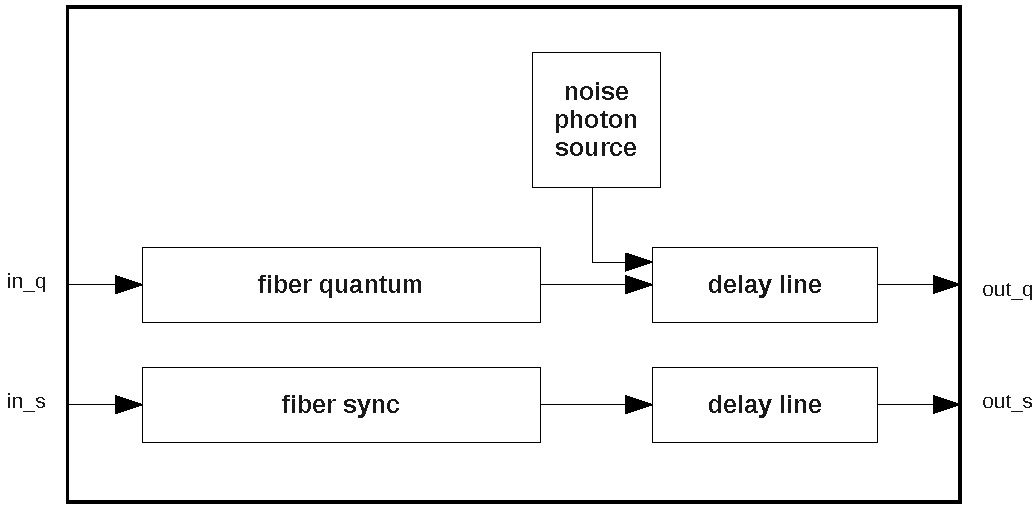
\includegraphics[scale=0.65]{drawings/fiber.pdf}
\caption{The transmission fiber}
\label{fig:outline_fiber}
\end{figure}

The transmission of photons is modelled to occur over a quantum transmission fiber (\textbf{fiber quantum}) and the transmission of the sync pulse over a sync pulse transmission fiber (\textbf{fiber sync}), although in reality they are both transmitted over the same fiber but at another wavelength using wavelength-division multiplexing (WDM) as already mentioned in section \ref{sec:overview}. There are also two \textbf{delay line}s that allow to model delay times between the photons and the sync pulse so that the photons arrive at Bob's detector later or earlier than the sync pulse. Also there is shown a \textbf{noise photon source} that is used for simulating stray light photons interspersed into the quantum transmission fiber. Photons generated by the \textbf{noise photon source} are stored as \texttt{photon\_pair} objects (see section \ref{subsec:concepts_photons}) where \texttt{m\_eStateA} is set to \texttt{ABSORBED} and \texttt{m\_eStateB} is set to \texttt{NONPOLARIZED}.

\subsection{Detector at Alice's Side}
\label{subsec:outline_detector_alice}

The different components of the detector at Alice's side are shown in Figure \ref{fig:outline_detector_alice} and will now be briefly described.

\begin{figure}[h]
\centering
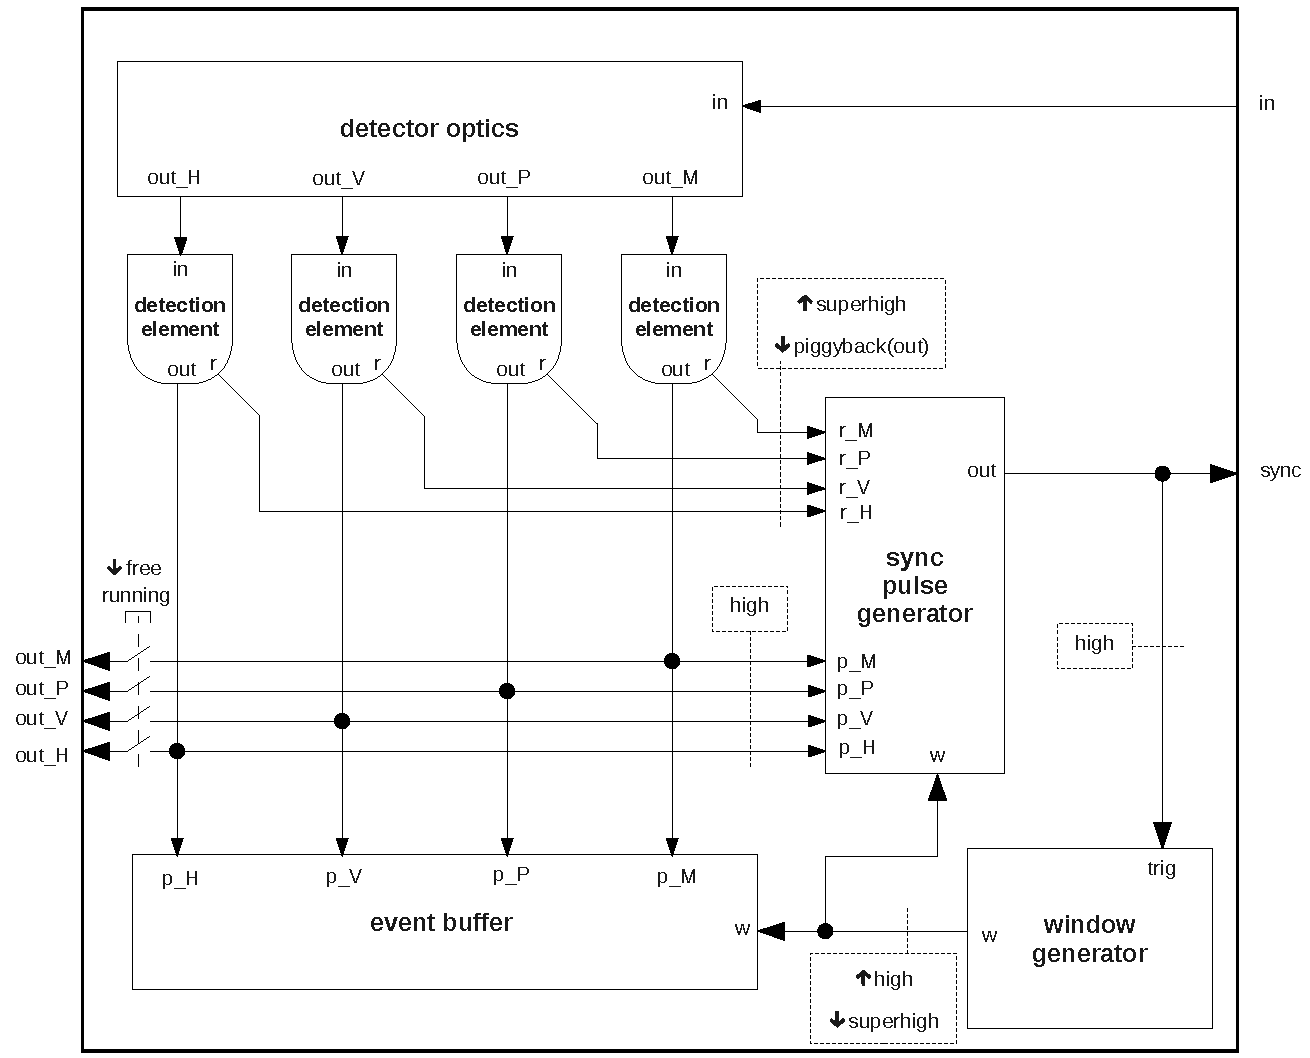
\includegraphics[scale=0.65]{drawings/detector_alice.pdf}
\caption{The detector at Alice's side}
\label{fig:outline_detector_alice}
\end{figure}

The \textbf{detector optics} component's purpose is to model optical components in the BB84 detector such as polarising and non-polarising beam splitters. When it receives an incident \texttt{photon} event, it makes random choices to decide to which of the four \textbf{detection element}s an incoming \texttt{photon} event will be sent, where the probabilities of the photon being forwarded to the specific \textbf{detection element}s are chosen depending on the incoming photon's polarisation in such a way that they reproduce the behaviour of the modelled BB84 detector.

The \textbf{detection element}s represent the four single photon detectors. Whenever they receive and detect a photon they generate an electrical \texttt{pulse} event. What happens next depends on which detection mode has been configured. There are four different modes available for Alice's detector:

\begin{itemize}

\item \textit{free running mode}: The electrical \texttt{pulse} events generated by the \textbf{detection element}s are forwarded by \textbf{detector alice} to \textbf{channel} and further to the \textbf{TTM} module (see Figure \ref{fig:quantum_channel}) which records the received events to a logging file named \texttt{TTM.log}.

\item \textit{sync mode}: The electrical \texttt{pulse} events generated by the \textbf{detection element}s are sent to the \textbf{sync pulse generator} and to the \textbf{event buffer}. As can be seen in Figure \ref{fig:outline_detector_alice}, the \texttt{pulse} event sent to the sync pulse generator is assigned \texttt{high} priority so that is arrives before the \textbf{event buffer} receives the \texttt{pulse} event. A second output each \textbf{detection element} provides is the `ready'' output (labelled with ``r'') that informs the \textbf{sync pulse generator} if the \textbf{detection element}s are in ready or down state. If a ``down time'' parameter has been configured for the \textbf{detection element}s, this means that whenever they receive a photon, they go into down state, and after some down time has passed, they go back into ready state. 
The beginning of a down period is indicated to the \textbf{sync pulse generator} by a flag transmitted together with the output \texttt{pulse} event - this is the reason why a downward arrow with the text ``piggyback(out)'' is shown in Figure \ref{fig:outline_detector_alice}. In this case, it exceptionally does not indicate the priority of a newly generated event but signifies that the information that a falling edge at the ``ready'' output occurred is transported piggyback by a flag included in the \texttt{pulse} output event. In the other case, however, that a rising edge occurs at the ``ready'' output (after the down time is over) an extra event of type \texttt{down\_end} with \texttt{superhigh} priority is generated and sent to the \textbf{sync pulse generator}.

Whenever the \textbf{sync pulse generator} receives a \texttt{pulse} event from a \textbf{detection element}, it checks if the \textbf{window generator} is currently ready (it has finished generating its last window, if one was triggered), and if it is, the \textbf{sync pulse generator} generates a \texttt{SYNC\_PULSE} event with \texttt{high} priority that is on the one hand forwarded by \textbf{detector alice} to \textbf{channel} and then further to \textbf{fiber}, and on the other hand it triggers the \textbf{window generator} to generate a new window of specified duration.

The rising edge of the \textbf{window generator}'s output signal (= the beginning of the new window) is signalled as a \texttt{high} priority event of type \texttt{WINDOW\_START} to the \textbf{event buffer}. The \textbf{event buffer} in turn hereupon clears its 4-bit-wide event latch and opens it to receive and store \texttt{pulse} events coming from the \textbf{detection element}s. Whenever further some \texttt{pulse} event coming from a \textbf{detection element} is send to the \textbf{event buffer} while its event latch is open, it stores a ``1'' for the bit in the event latch corresponding to the respective \textbf{detection element}. 

This now shows the reason why \texttt{high} priority events are necessary for the \texttt{pulse} event send from the \textbf{detection element}s to the \textbf{sync pulse generator} and from the \textbf{sync pulse generator} to the \textbf{window generator} as well as for the \texttt{WINDOW\_START} event sent to the \textbf{event buffer}: It must be ensured that a \texttt{pulse} event coming from a \textbf{detection element} that triggers a new window can open the \textbf{event buffer}s event latch first before the \texttt{pulse} event itself is sent to the \texttt{event buffer} so that it gets stored in the event latch. 

After some time, the \textbf{window generator} closes its window and signals the falling edge of the window output signal by sending a \texttt{WINDOW\_END} event of \texttt{superhigh} priority to the \textbf{event buffer} and the \textbf{sync pulse generator}, which causes the \textbf{event buffer} to close its event latch and write its contents to a key buffer, and also informs the \textbf{sync pulse generator} that the \textbf{window generator} is now ready to generate a new window. The \texttt{superhigh} priority is used for the \texttt{WINDOW\_END} event because in the case that at the same time a new \texttt{pulse} event comes from a \textbf{detection element}, it shall be ensured that at first the \textbf{event buffer} and the \textbf{sync pulse generator} are informed that the previous window has been closed.

\item \textit{sync mode - wait for sync initiator to be ready}: The behaviour of \textbf{detector alice} is almost the same as in \textit{sync mode}, with the only difference that whenever the \textbf{sync pulse generator} generates a sync pulse, it remembers which of the four \textbf{detection element}s was the initiator of the sync pulse, and in the case that the initiating \textbf{detection element} goes into down state after sending the \texttt{pulse} event, the \textbf{sync pulse generator} does not generate new sync pulses until the initiating \textbf{detection element} goes back into ready state.

\item \textit{sync mode - wait for all detection elements to be ready}: The behaviour of \textbf{detector alice} is almost the same as in \textit{sync mode}, with the only difference that the \textbf{sync pulse generator} does only generate a sync pulse if all \textbf{detection element}s are in ready state (none of them is down).

\end{itemize}

\subsection{Detector at Bob's Side}
\label{subsec:outline_detector_bob}

The detector at Bob's side with its components is shown in Figure \ref{fig:outline_detector_bob}. It looks very similar to that at Alice's side, with the difference that instead of a \textbf{sync pulse generator} it contains a \textbf{sync pulse receiver}, and the \textbf{detection element}s, the \textbf{window generator} and the \textbf{event buffer} have some extra input and output signals (bad, bad\_out).

\begin{figure}[h]
\centering
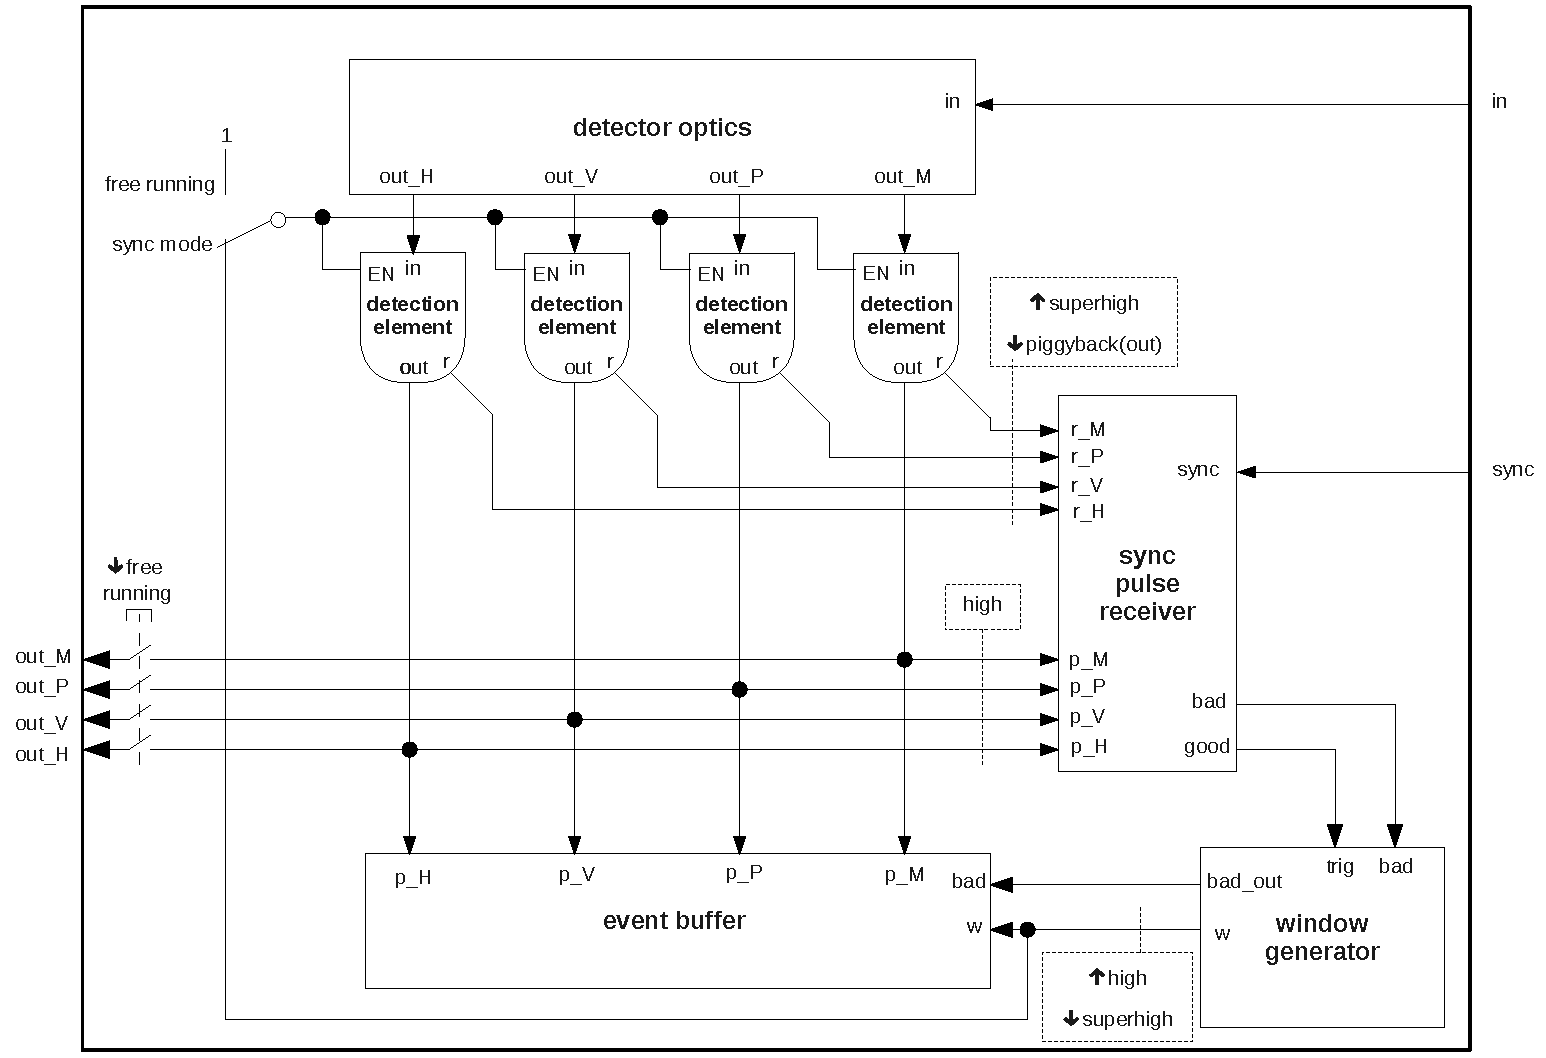
\includegraphics[scale=0.65]{drawings/detector_bob.pdf}
\caption{The detector at Bob's side}
\label{fig:outline_detector_bob}
\end{figure}

The behaviour of many parts of \textbf{detector bob} is the same as for \textbf{detector alice} - therefore, only the differences are described now. There are three possible operation modes for \textbf{detector bob}:

\begin{itemize}

\item \textit{free running mode}: In this mode, \textbf{detector bob} behaves exactly in the same way as \textbf{detector alice} does. Additionally it must be noted that in this mode, the delay time for the delay line connected to the output of the quantum transmission fiber (see Figure \ref{fig:outline_fiber}) is set to zero, so that when all system components parameters are configured for the ideal case, the same detection times are recorded by the TTM for the two photons (travelling to Alice and Bob) belonging to one entangled photon pair.

\item \textit{sync mode}: Whenever the \textbf{sync pulse receiver} receives a \texttt{SYNC\_PULSE} event (that originally came from \textbf{detector alice}'s \textbf{sync pulse generator} and travelled over the \textbf{fiber}) it triggers the window generator by sending a \texttt{SYNC\_PULSE} event to it. The \textbf{window generator} in turn sends a \texttt{WINDOW\_START} event to the \textbf{event buffer}. In the case that there was already a window opened by the \textbf{window generator} and has not been closed before, the \textbf{window generator} newly calculates when the \texttt{WINDOW\_END} event should occur (according to the configured window duration). 

The \textbf{detection element}s operate in a ``gated'' mode - they are only enabled to receive photons when the \textbf{window generator}'s output is currently in high state (which means that a window is currently open).

The \textbf{event buffer} operates in the same way is in \textbf{detector alice}, but with the additional feature that when it receives a \texttt{WINDOW\_START} event when its event latch is already open (no \texttt{WINDOW\_END} event came after the previous \texttt{WINDOW\_START} event), it writes the current contents of the event latch to the key buffer, clears the event latch and the event latch remains in opened state.

\item \textit{sync mode - wait for all detection elements to be ready}: The \textbf{detector bob} operates similarly as in \textit{sync mode} but with some differences and enhancements: In the case that the \textbf{sync pulse receiver} receives a \texttt{SYNC\_PULSE} event while not all \textbf{detection element}s are in ready state, it sends a \texttt{SYNC\_PULSE\_BAD} event instead of a \texttt{SYNC\_PULSE} event to the \textbf{window generator}. 

When the \textbf{window generator} receives the \texttt{SYNC\_PULSE\_BAD} event, how it acts depends on its current state: If no window is open currently, the \textbf{window generator} sends a \texttt{SYNC\_PULSE\_BAD} event to the \textbf{event buffer}. If a window is currently open, however, the \textbf{window generator} closes the active window and sends a \texttt{window\_end\_bad} event to the \textbf{event buffer}.

The \textbf{event buffer}, when it receives a \texttt{SYNC\_PULSE\_BAD} event, writes a zero entry to the key buffer. When the \textbf{event buffer} receives a \texttt{window\_end\_bad} event, it first closes its event latch and writes the current contents of the event latch to the key buffer, then it additionally writes a zero entry to the key buffer.

\end{itemize}


\newpage
\section{Components of the QKD Simulator}
\label{sec:comp}

In this section, the components of the QKD simulator are described in greater detail. It should be mentioned that the descriptions in this section neither cover all aspects of the components' implementations in the C++11 code nor follow these implementations rigorously, but have the intention to provide a simplified breakdown of the components' functions.

\subsection{\texttt{channel}}
\label{subsec:comp_channel}

\textbf{Short description:}\\
This components simulates the quantum channel. \\
\\
\textbf{Defined in files:}\\
\texttt{channel/channel.h}\\
\texttt{channel/channel.cpp}\\
\\
\textbf{Properties:}
\begin{lstlisting}
double m_nStndSyncDeviation;    /**< Standard deviation for the Gaussian
                                     sync signal stored in unit [ns], 
                                     range [0-100 ns] */
double m_nTimeslotCenterShift;  /**< timeslot center shift in [ns] */
\end{lstlisting}
\noindent
\textbf{Subcomponents:}
\begin{lstlisting}
channel_event_manager m_cManager;           /**< the channel event manager */
photon_pair_manager m_cPhotonPairManager;  /**< the photon pair manager */
detector * m_cDetectorAlice;               /**< alice detector */
detector * m_cDetectorBob;                 /**< bob detector */
fiber m_cFiber;                            /**< the transmission medium */
source m_cSource;                          /**< quantum source */
ttm m_ttm;                                 /**< the TTM module */
\end{lstlisting}
\noindent
\textbf{Component behaviour for parameter configuration:}
\begin{itemize}

\item If the \texttt{m\_nStndSyncDeviation} property is changed to value \texttt{nStndDeviation}, then the following changes happen:

\begin {itemize}

\item \texttt{m\_cDetectorBob->m\_cSyncPulseReceiver.m\_nJitter} is set to \texttt{nStndDeviation}

\item \texttt{m\_cDetectorBob->m\_cSyncPulseReceiver.m\_nDelay} is set to \texttt{5.0 * nStndDeviation}

\item \texttt{update\_delay\_times()} is called

\end {itemize}

\item If the \texttt{m\_nTimeslotCenterShift} property is changed, then \texttt{update\_delay\_times()} is called.

\item Behaviour of \texttt{update\_delay\_times()}:

\begin{itemize}

\item If the simulation is in \textit{free running mode}, \texttt{m\_cFiber.m\_cDelayLine.m\_nDelayTime} and \texttt{m\_cFiber.m\_cDelayLineSync.m\_nDelayTime} are set to 0

\item If the simulation is not in \textit{free running mode}, a \texttt{double} variable \texttt{delay} is calculated as \\
\\
\texttt{delay = 5.0 * m\_nStndSyncDeviation + 0.5 * m\_cDetectorBob->time\_slot\_width() + m\_nTimeslotCenterShift;}\\
\\
and \texttt{m\_cFiber.m\_cDelayLine.m\_nDelayTime} is set to \texttt{max(delay, 0.0)} and \texttt{m\_cFiber.m\_cDelayLineSync.m\_nDelayTime} is set to \texttt{max(-delay, 0.0)}

\end{itemize}

\end{itemize}
\noindent
\textbf{Component behaviour during simulation:}\\
Event forwarding is performed according to Table \ref{tab:comp_channel_evfwd}.

\begin{table}[H]
\begin{tabular}{ | l | l || l | l | p{4cm} | }
\hline
\multicolumn{1}{|c|}{\textbf{Event type}} & \multicolumn{1}{c||}{\textbf{Source}} & \multicolumn{1}{c|}{\textbf{Destination}} & \multicolumn{1}{c|}{\textbf{new priority}} & \multicolumn{1}{c|}{\textbf{new \texttt{m\_cData} values}} \\
\hline \hline
\texttt{photon} & \texttt{m\_cSource} & \texttt{m\_cDetectorAlice} &  & \\
\cline{3-5}
 & & \texttt{m\_cFiber} & \texttt{subnormal} & \\
\cline{2-5}
 & \texttt{m\_cFiber} & \texttt{m\_cDetectorBob} & & \\
\hline
\texttt{detector\_pulse} & \texttt{m\_cDetectorAlice} & \texttt{m\_cTTM} & & \texttt{m\_bAlice = true;} \\
\cline{2-5}
 & \texttt{m\_cDetectorBob} & \texttt{m\_cTTM} & & \texttt{m\_bAlice = false;} \\
\hline
\texttt{sync\_pulse} & \texttt{m\_cDetectorAlice}  & \texttt{m\_cFiber} & & \\
\cline{2-5}
 & \texttt{m\_cFiber}  & \texttt{m\_cDetectorBob} & & \\
\hline
\end{tabular}
\caption{Event forwarding in the \texttt{channel} component}
\label{tab:comp_channel_evfwd}
\end{table}

\subsubsection{\texttt{detector}}
\label{subsubsec:comp_detector}

\textbf{Short description:}\\
This component simulates the BB84 detector module.\\
\\
\textbf{Defined in files:}\\
\texttt{channel/detector.h}\\
\texttt{channel/detector.cpp}\\
\\
\textbf{Properties:}
\begin{lstlisting}
bool m_bAlice;                     /**< state if we are alice */
bool m_bDarkCounts;                /**< dark counts enabled */
detection_mode m_eDetectionMode;   /**< detection mode for this detector */
double m_nDarkCountRate;           /**< dark count rate in 1/s */
double m_nDownTime;                /**< down time in ns */
double m_nEfficiency;              /**< efficiency [0 - 1] */
uint64_t m_nEventTableSize;        /**< event table size in bytes */
bool m_bJitter;                    /**< jitter enabled */
bool m_bLoss;                      /**< loss enabled */
double m_nLossRate;                /**< distance independent loss in 
                                        dB/km */
double m_nPhotonTimeDelay;         /**< photon detection time delay in ns */
double m_nPhotonTimeStndDeviation; /**< photon time standard deviation 
                                        in ns */
double m_nTimeSlotWidth;           /**< time slot width == coincidence
                                        window in ns */
\end{lstlisting}
\noindent
\textbf{Subcomponents:}
\begin{lstlisting}
detector_optics m_cDetectorOptics;             /**<the detector optics */
detection_element m_cDetectionElementH;       /**< detection element for
                                                    horizontal polarization */
detection_element m_cDetectionElementV;       /**< detection element for
                                                    vertical polarization */
detection_element m_cDetectionElementP;       /**< detection element for
                                                    "plus" polarization */
detection_element m_cDetectionElementM;       /**< detection element for
                                                    "minus" polarization */
event_buffer m_cEventBuffer;                   /**< event buffer */
sync_pulse_generator * m_cSyncPulseGenerator; /**< sync pulse generator
                                                    (only used at Alice's
                                                    side) */
sync_pulse_receiver * m_cSyncPulseReceiver;   /**< sync pulse receiver
                                                    (only used at Bob's
                                                    side) */
window_generator m_cWindowGenerator;           /**< window generator */
\end{lstlisting}
\noindent
\\
The \texttt{m\_eDetectionMode} property must be set to one of the constants defined in \texttt{channel/detector/detection\_modes.h} (see Listing \ref{lst:detection_mode}).

\begin{lstlisting}[caption={Definition of the \texttt{detection\_mode} enumeration type}, captionpos=b, label={lst:detection_mode}]
enum struct detection_mode {
    free_running,        /**< detector is free running (no sync pulse
                              generation/receive, only TTM records) */
    sync,                /**< sync pulse generation/receive irrespective of
                              detector down times */
    sync_initiator_ready /**< mode valid only for Alice side: sync pulse
                              generation, but only if last sync pulse initiator is not down anymore */,
    sync_all_ready       /**< meaning at Alice side: sync pulse generation,
                              but only if no detection element is down.
                           *  meaning at Bob side:   sync pulse receive, but
                              if one or more detection elements are down, a zero entry is stored in event buffer */
};
\end{lstlisting}
\noindent
\textbf{Component behaviour for parameter configuration:}
\begin{itemize}

\item If the \texttt{m\_bDarkCounts} or \texttt{m\_nDarkCountRate} property is changed, \texttt{update\_dark\_count\_rate()} is called.

\item If the \texttt{m\_eDetectionMode} parameter is changed, the following steps are performed:

\begin{itemize}

\item If the \texttt{m\_bAlice} property is \texttt{true} or \texttt{m\_eDetectionMode} is set to \texttt{free\_running}, the \texttt{m\_init\_enabled} property of
all four \texttt{detection\_element} subcomponents is set to \texttt{true}, otherwise, it is set to \texttt{false}.

\item If the \texttt{m\_bAlice} property is \texttt{true}, \texttt{m\_cSyncPulseGenerator->\-m\_eDetectionMode} is set to the new \texttt{m\_eDetectionMode} value, otherwise, \texttt{m\_cSyncPulseReceiver->\-m\_eDetectionMode} is set to the new \texttt{m\_eDetectionMode} value.

\end{itemize}

\item If the \texttt{m\_bLoss}, \texttt{m\_nDownTime}, \texttt{m\_nEfficiency} or \texttt{m\_nLossRate} property is changed, \texttt{update\_detection\_loss()} is called.

\item If the \texttt{m\_nEventTableSize} property is changed, \texttt{m\_event\_buffer.m\_nBufferSize} is updated to the new value.

\item If the \texttt{m\_bJitter}, \texttt{m\_nPhotonTimeDelay} or \texttt{m\_nPhotonTimeStndDeviation} property is changed, \texttt{update\_jitter()} is called.

\item If the \texttt{m\_nTimeSlotWidth} property is changed, \texttt{m\_window\_generator.m\_window\_width} is updated to the new value.

\item Behaviour of \texttt{update\_dark\_count\_rate()}:

\begin{itemize}

\item If \texttt{m\_bDarkCounts} is \texttt{true}, the \texttt{m\_nDarkCountRate} property of all four \texttt{detection\_element} subcomponents is set to \texttt{m\_nDarkCountRate}

\item If \texttt{m\_bDarkCounts} is \texttt{false}, the \texttt{m\_nDarkCountRate} property of all four \texttt{detection\_element} subcomponents is set to 0

\end{itemize}

\item Behaviour of \texttt{update\_detection\_loss()}:

\begin{itemize}

\item If \texttt{m\_bLoss} is \texttt{true}, the \texttt{m\_nLoss} property of the \texttt{m\_cDetectorOptics} subcomponent is set to \texttt{m\_nLossRate}, the \texttt{m\_nEfficiency} property of the \texttt{m\_cDetectorOptics} subcomponent is set to \texttt{m\_nEfficiency}, and the \texttt{m\_bDown\_time} of all four \texttt{detection\_element} subcomponents is set to \texttt{m\_nDownTime}.

\item If \texttt{m\_bLoss} is \texttt{false}, the \texttt{m\_nLoss} property of the \texttt{m\_cDetectorOptics} subcomponent is set to 0, the \texttt{m\_nEfficiency} property of the \texttt{m\_cDetectorOptics} subcomponent is set to 1, and the \texttt{m\_bDown\_time} of all four \texttt{detection\_element} subcomponents is set to 0.

\end{itemize}

\item Behaviour of \texttt{update\_jitter()}:

\begin{itemize}

\item If \texttt{m\_bJitter} is \texttt{true}, for all four \texttt{detection\_element} subcomponents the \texttt{m\_nDelay} property is set to \texttt{m\_nPhotonTimeDelay}, and the \texttt{m\_nJitter} property is set to \texttt{m\_nPhotonTimeStndDeviation}.

\item If \texttt{m\_bJitter} is \texttt{false}, for all four \texttt{detection\_element} subcomponents the \texttt{m\_nDelay} and \texttt{m\_nJitter} properties are set to 0.

\end{itemize}

\end{itemize}
\noindent
\textbf{Component behaviour during simulation:}\\
This component does event forwarding as described in Table \ref{tab:comp_detector_evfwd}.

\begin{footnotesize}
\begin{longtable}[H]{ | m{1.2cm} | m{1.9cm} | m{1.2cm} | l | m{1.5cm} || m{1.8cm} | m{1.4cm} | m{1.2cm} | m{1.7cm} | }
\captionsetup{font=normalsize}
\hline
  \multicolumn{1}{| >{\centering}p{1cm}<{\centering} |}{\textbf{Event} \par \textbf{type}} & 
  \multicolumn{1}{c|}{\textbf{Source}} & 
  \multicolumn{1}{ >{\centering}p{1.2cm}<{\centering} |}{\textbf{free} \par \textbf{running}} &
  \multicolumn{1}{c|}{\textbf{\texttt{m\_bAlice}}} &
  \multicolumn{1}{ >{\centering}p{1.5cm}<{\centering} ||}{\textbf{Incoming} \par \textbf{\texttt{m\_cData}}} & 
  \multicolumn{1}{c|}{\textbf{Destination}} & 
  \multicolumn{1}{ >{\centering}p{1.4cm}<{\centering} |}{\textbf{New type}} & 
  \multicolumn{1}{ >{\centering}p{1.2cm}<{\centering} |}{\textbf{New} \par \textbf{priority}} & 
  \multicolumn{1}{ >{\centering}p{1.7cm}<{\centering} |}{\textbf{New} \par \textbf{\texttt{m\_cData}}} \\
\hline \hline
  \texttt{down\_end} &
  \texttt{m\_cDetectionElementH} &
  \texttt{false} &
  \texttt{false} &
  &
  \texttt{m\_cSyncPulseReceiver} &
  &
  &
  \texttt{m\_phs =} \par \texttt{horizontal;} \\
\cline{4-9}
  & 
  & 
  & 
  \texttt{true} & 
  & 
  \texttt{m\_cSyncPulseGenerator} & 
  & 
  & 
  \texttt{m\_phs =} \par \texttt{horizontal;} \\ 
\cline{2-9}
  &
  \texttt{m\_cDetectionElementV} &
  \texttt{false} &
  \texttt{false} &
  &
  \texttt{m\_cSyncPulseReceiver} &
  &
  &
  \texttt{m\_phs =} \par \texttt{vertical;} \\
\cline{4-9}
  & 
  & 
  & 
  \texttt{true} & 
  &
  \texttt{m\_cSyncPulseGenerator} & 
  & 
  & 
  \texttt{m\_phs =} \par \texttt{vertical;} \\
\cline{2-9}
  &
  \texttt{m\_cDetectionElementP} &
  \texttt{false} &
  \texttt{false} &
  &
  \texttt{m\_cSyncPulseReceiver} &
  &
  &
  \texttt{m\_phs =} \par \texttt{plus;} \\
\cline{4-9}
  &
  &
  &
  \texttt{true} &
  &
  \texttt{m\_cSyncPulseGenerator} &
  &
  &
  \texttt{m\_phs =} \par \texttt{plus;} \\
\cline{2-9}
  &
  \texttt{m\_cDetectionElementM} &
  \texttt{false} &
  \texttt{false} &
  &
  \texttt{m\_cSyncPulseReceiver} &
  &
  &
  \texttt{m\_phs =} \par \texttt{minus;} \\
\cline{4-9}
  &
  &
  &
  \texttt{true} &
  &
  \texttt{m\_cSyncPulseGenerator} &
  &
  &
  \texttt{m\_phs =} \par \texttt{minus;} \\
  
\hline

  \texttt{photon} &
  parent &
  &
  &
  &
  \texttt{m\_detector\_} \par \texttt{optics} &
  &
  \texttt{normal} &
  \\
\cline{2-9}
  &
  \texttt{m\_detector\_} \par \texttt{optics} &
  &
  &
  \texttt{m\_phs ==} \par \texttt{horizontal} &
  \texttt{m\_cDetectionElementH} &
  &
  &
  \\
\cline{5-9}
  &
  &
  &
  &
  \texttt{m\_phs ==} \par \texttt{vertical} &
  \texttt{m\_cDetectionElementV} &
  &
  &
  \\
\cline{5-9}
  &
  &
  &
  &
  \texttt{m\_phs ==} \par \texttt{plus} &
  \texttt{m\_cDetectionElementP} &
  &
  &
  \\
\cline{5-9}
  &
  &
  &
  &
  \texttt{m\_phs ==} \par \texttt{minus} &
  \texttt{m\_cDetectionElementM} &
  &
  &
  \\
  
\hline

  \texttt{pulse} &
  \texttt{m\_cDetectionElementH} &
  \texttt{false} &
  &
  &
  \texttt{m\_cEventBuffer} &
  \texttt{detector\_} \par \texttt{pulse} &
  &
  \texttt{m\_phs =} \par \texttt{horizontal;} \\
\cline{4-9}
  &
  &
  &
  \texttt{false} &
  &
  \texttt{m\_cSyncPulseReceiver} &
  \texttt{detector\_} \par \texttt{pulse} &
  \texttt{high} &
  \texttt{m\_phs =} \par \texttt{horizontal;} \\
\cline{4-9}
  &
  &
  &
  \texttt{true} &
  &
  \texttt{m\_cSyncPulseGenerator} &
  \texttt{detector\_} \par \texttt{pulse} &
  \texttt{high} &
  \texttt{m\_phs =} \par \texttt{horizontal;} \\
\cline{3-9}
  &
  &
  \texttt{true} &
  &
  &
  parent &
  \texttt{detector\_} \par \texttt{pulse} &
  &
  \texttt{m\_phs =} \par \texttt{horizontal;} \\
\cline{2-9}
  &
  \texttt{m\_cDetectionElementV} &
  \texttt{false} &
  &
  &
  \texttt{m\_cEventBuffer} &
  \texttt{detector\_} \par \texttt{pulse} &
  &
  \texttt{m\_phs =} \par \texttt{vertical;} \\
\cline{4-9}
  &
  &
  &
  \texttt{false} &
  &
  \texttt{m\_cSyncPulseReceiver} &
  \texttt{detector\_} \par \texttt{pulse} &
  \texttt{high} &
  \texttt{m\_phs =} \par \texttt{vertical;} \\
\cline{4-9}
  &
  &
  &
  \texttt{true} &
  &
  \texttt{m\_cSyncPulseGenerator} &
  \texttt{detector\_} \par \texttt{pulse} &
  \texttt{high} &
  \texttt{m\_phs =} \par \texttt{vertical;} \\
\cline{3-9}
  &
  &
  \texttt{true} &
  &
  &
  parent &
  \texttt{detector\_} \par \texttt{pulse} &
  &
  \texttt{m\_phs =} \par \texttt{vertical;} \\
\cline{2-9}
  &
  \texttt{m\_cDetectionElementP} &
  \texttt{false} &
  &
  &
  \texttt{m\_cEventBuffer} &
  \texttt{detector\_} \par \texttt{pulse} &
  &
  \texttt{m\_phs =} \par \texttt{plus;} \\
\cline{4-9}
  &
  &
  &
  \texttt{false} &
  &
  \texttt{m\_cSyncPulseReceiver} &
  \texttt{detector\_} \par \texttt{pulse} &
  \texttt{high} &
  \texttt{m\_phs =} \par \texttt{plus;} \\
\cline{4-9}
  &
  &
  &
  \texttt{true} &
  &
  \texttt{m\_cSyncPulseGenerator} &
  \texttt{detector\_} \par \texttt{pulse} &
  \texttt{high} &
  \texttt{m\_phs =} \par \texttt{plus;} \\
\cline{3-9}
  &
  &
  \texttt{true} &
  &
  &
  parent &
  \texttt{detector\_} \par \texttt{pulse} &
  &
  \texttt{m\_phs =} \par \texttt{plus;} \\
\cline{2-9}
  &
  \texttt{m\_cDetectionElementM} &
  \texttt{false} &
  &
  &
  \texttt{m\_cEventBuffer} &
  \texttt{detector\_} \par \texttt{pulse} &
  &
  \texttt{m\_phs =} \par \texttt{minus;} \\
\cline{4-9}
  &
  &
  &
  \texttt{false} &
  &
  \texttt{m\_cSyncPulseReceiver} &
  \texttt{detector\_} \par \texttt{pulse} &
  \texttt{high} &
  \texttt{m\_phs =} \par \texttt{minus;} \\
\cline{4-9}
  &
  &
  &
  \texttt{true} &
  &
  \texttt{m\_cSyncPulseGenerator} &
  \texttt{detector\_} \par \texttt{pulse} &
  \texttt{high} &
  \texttt{m\_phs =} \par \texttt{minus;} \\
\cline{3-9}
  &
  &
  \texttt{true} &
  &
  &
  parent &
  \texttt{detector\_} \par \texttt{pulse} &
  &
  \texttt{m\_phs =} \par \texttt{minus;} \\
  
\hline

  \texttt{sync\_} \par \texttt{pulse} &
  parent &
  &
  \texttt{false} &
  &
  \texttt{m\_cSyncPulseReceiver} &
  &
  &
  \\
\cline{2-9}
  &
  \texttt{m\_cSyncPulseReceiver} &
  &
  \texttt{false} &
  &
  \texttt{m\_cWindowGenerator} &
  &
  &
  \\
\cline{2-9}
  &
  &
  &
  \texttt{true} &
  &
  parent &
  &
  &
  \\
\cline{6-9}
  &
  &
  &
  &
  &
  \texttt{m\_cWindowGenerator} &
  &
  \texttt{high} &
  \\
  
\hline

  \texttt{sync\_} \par \texttt{pulse\_} \par \texttt{bad} &
  \texttt{m\_cSyncPulseReceiver} &
  &
  &
  &
  \texttt{m\_cWindowGenerator} &
  &
  &
  \\
\cline{2-9}
  &
  \texttt{m\_cWindowGenerator} &
  &
  &
  &
  \texttt{m\_cEventBuffer} &
  &
  &
  \\
  
\hline

  \texttt{window\_} \par \texttt{end} &
  &
  &
  &
  &
  \texttt{m\_cEventBuffer} &
  &
  &
  \\
\cline{4-9}
  &
  &
  &
  \texttt{false} &
  &
  \texttt{m\_cDetectionElementH} &
  \texttt{disable} &
  &
  \\
\cline{6-9}
  &
  &
  &
  &
  &
  \texttt{m\_cDetectionElementV} &
  \texttt{disable} &
  &
  \\
\cline{6-9}
  &
  &
  &
  &
  &
  \texttt{m\_cDetectionElementP} &
  \texttt{disable} &
  &
  \\
\cline{6-9}
  &
  &
  &
  &
  &
  \texttt{m\_cDetectionElementM} &
  \texttt{disable} &
  &
  \\
\cline{4-9}
  &
  &
  &
  \texttt{true} &
  &
  \texttt{m\_cSyncPulseGenerator} &
  &
  &
  \\
  
\hline

  \texttt{window\_} \par \texttt{end\_bad} &
  &
  &
  &
  &
  \texttt{m\_cEventBuffer} &
  &
  &
  \\
\cline{6-9}
  &
  &
  &
  &
  &
  \texttt{m\_cDetectionElementH} &
  \texttt{disable} &
  &
  \\
\cline{6-9}
  &
  &
  &
  &
  &
  \texttt{m\_cDetectionElementV} &
  \texttt{disable} &
  &
  \\
\cline{6-9}
  &
  &
  &
  &
  &
  \texttt{m\_cDetectionElementP} &
  \texttt{disable} &
  &
  \\
\cline{6-9}
  &
  &
  &
  &
  &
  \texttt{m\_cDetectionElementM} &
  \texttt{disable} &
  &
  \\
  
\hline

  \texttt{window\_} \par \texttt{start} &
  &
  &
  &
  &
  \texttt{m\_cEventBuffer} &
  &
  &
  \\
\cline{4-9}
  &
  &
  &
  \texttt{false} &
  &
  \texttt{m\_cDetectionElementH} &
  \texttt{enable} &
  &
  \\
\cline{6-9}
  &
  &
  &
  &
  &
  \texttt{m\_cDetectionElementV} &
  \texttt{enable} &
  &
  \\
\cline{6-9}
  &
  &
  &
  &
  &
  \texttt{m\_cDetectionElementP} &
  \texttt{enable} &
  &
  \\
\cline{6-9}
  &
  &
  &
  &
  &
  \texttt{m\_cDetectionElementM} &
  \texttt{enable} &
  &
  \\
\hline
\caption{Event forwarding in the \texttt{detector} component}
\label{tab:comp_detector_evfwd}
\end{longtable}
\end{footnotesize}

\paragraph{\texttt{detection\_element}}
\label{par:comp_detector_detelem}
\noindent \\
\\
\textbf{Short description:}\\
This component simulates the single photon detection element.\\
\\
\textbf{Defined in files:}\\
\texttt{channel/detector/detection\_element.h}\\
\texttt{channel/detector/detection\_element.cpp}\\
\\
\textbf{Properties:}
\begin{lstlisting}
double   m_nDarkCountRate;  /**< dark count rate in 1/s */
double   m_nDelay;          /**< delay in ns */
bool     m_bDown;           /**< states whether this detection element is
                                 down */
double   m_nDownTime;       /**< down time in ns */
bool     m_bEnabled;        /**< states whether this detection element is
                                 enabled */
bool     m_bInitEnabled;    /**< states whether this detection element is
                                 enabled at initialization */
double   m_nJitter;         /**< jitter in ns */
\end{lstlisting}
\noindent
\textbf{Component behaviour during simulation:}
\begin{itemize}

\item When an \texttt{init} event is received, \texttt{m\_bDown} is set to \texttt{false}, \texttt{m\_bEnabled} is set to \texttt{m\_init\_enabled}, and \texttt{add\_next\_dark\_count\_event()} is called.

\item When an \texttt{enable} event is received, \texttt{m\_bEnabled} is set to \texttt{true}.

\item When a \texttt{disable} event is received, \texttt{m\_bEnabled} is set to \texttt{false}.

\item When a \texttt{photon} event is received and at this time \texttt{m\_bEnabled} is \texttt{true} and \texttt{m\_bDown} is \texttt{false}, a new event of type \texttt{detect} is created and sent to this component, with the event time set to occur after some delay time \texttt{td}, that is calculated as the sum of \texttt{m\_nDelay} plus a random value of Gaussian distribution with mean value 0 and standard deviation \texttt{m\_nJitter}, but \texttt{td} is constrained to be non-negative - if it is negative, the jitter random value is ``reshuffled'' until \texttt{td} is non-negative.

\item When a \texttt{detect} event is received and at this time \texttt{m\_bEnabled} is \texttt{true} and \texttt{m\_bDown} is \texttt{false}, a new event of type \texttt{pulse} is created and sent to the parent event handler, with the new event's \texttt{m\_cData.m\_detect\_time} member set to the current simulation time and the \texttt{m\_cData.m\_bDown} member set to \texttt{true} if \texttt{m\_bDown\_time} is greater than 0 or to \texttt{false} otherwise.

Additionally, if \texttt{m\_bDown\_time} is greater than 0, \texttt{m\_bDown} is set to \texttt{true}, and a new event of type \texttt{down\_end} with \texttt{superhigh} priority is created and sent to this component, with its event time set to occur after a waiting time according to \texttt{m\_bDown\_time}.

\item When a \texttt{dark\_count} event is received, \texttt{add\_next\_dark\_count\_event()} is called to set the next dark count event, and then the same steps are performed as described for the case that a \texttt{detect} event is received.

\item When a \texttt{down\_end} event is received, \texttt{m\_bDown} is set to \texttt{false}, and a new event of type \texttt{down\_end} and of \texttt{superhigh} priority is created and sent to the parent event handler.

\item Behaviour of \texttt{add\_next\_dark\_count\_event()}:

\begin{itemize}

\item If \texttt{m\_nDarkCountRate} is greater than 0, a new event of type \texttt{dark\_count} with \texttt{m\_destination} set to this component is created, with the event time set to occur after some waiting period that is calculated at random using an exponential distribution with a mean value according to the \texttt{m\_nDarkCountRate} value.

\end{itemize}

\end{itemize}

\paragraph{\texttt{detector\_optics}}
\label{par:comp_detector_detopt}
\noindent \\
\\
\textbf{Short description:}\\
This component simulates the optical components of the BB84 detection module.\\
\\
\textbf{Defined in files:}\\
\texttt{channel/detector/detector\_optics.h}\\
\texttt{channel/detector/detector\_optics.cpp}\\
\\
\textbf{Properties:}
\begin{lstlisting}
bool   m_bAlice;              /**< states whether this detector_optics object
                                  is at Alice side */
double m_nDetectProbability;  /**< combined probability for photon detection
                                  [0 - 1] */
double m_nEfficiency;         /**< detection efficiency [0 - 1] */
double m_nLoss;               /**< loss in dB */
\end{lstlisting}
\noindent
\textbf{Component behaviour for parameter configuration:}
\begin{itemize}

\item If the \texttt{m\_nEfficiency} or \texttt{m\_nLoss} property is changed, \texttt{update\_detect\_probability()} is called.

\item Behaviour of \texttt{update\_detect\_probability()}:

\begin{itemize}

\item \texttt{m\_detect\_probability} is set to\\
\texttt{m\_nEfficiency * pow(10.0, -m\_nLoss / 10.0)}\\
where \texttt{pow} is the power function defined in \texttt{<cmath>}.

\end{itemize}

\end{itemize}
\noindent
\textbf{Component behaviour during simulation:}\\
Whenever the component receives an event \texttt{ev} of type \texttt{photon}, the following steps are performed, where \texttt{php} is a reference to the \texttt{photon\_pair} identified by \texttt{ev.m\_cData.m\_php\_id}:
\begin{enumerate}

\item Two pointers of type \texttt{photon\_state*} with names \texttt{phs\_here} and \texttt{phs\_there} are created. If \texttt{m\_bAlice} is \texttt{true}, they are set as follows:\\
\\
\texttt{phs\_here = \&(php.m\_eStateA);\\
phs\_there = \&(php.m\_eStateB);}\\
\\
otherwise, if \texttt{m\_bAlice} is \texttt{false}, they are set as:\\
\\
\texttt{phs\_here = \&(php.m\_eStateB);\\
phs\_there = \&(php.m\_eStateA);}\\

\item If \texttt{*phs\_here != absorbed}, the photon travelling to the ``here'' side will be detected with a probability of \texttt{m\_detect\_probability}, and in the case of detection, the following steps are performed:

\begin{enumerate}

\item A detected polarisation state for the ``here'' side is chosen randomly depending on \texttt{*phs\_here}, with probabilities for the different polarisations as shown in Table \ref{tab:comp_detector_detopt_prob}. The reason for the detection probabilities to be as shown in this table is that the H/V or P/M basis is chosen for measurement at random with equal probability, as already described in section \ref{sec:overview}.

\item A new event of type \texttt{photon} with its \texttt{m\_cData.m\_phs} member set according to the detected polarisation state is sent to the parent event handler.

\item If \texttt{*phs\_here} is equal to \texttt{entangled}, then \texttt{*phs\_there} is set with a probability of \texttt{(1.0 - php.entanglement\_error)} to the polarisation state orthogonal to that detected for the ``here'' side, or in the other case (of probability \texttt{php.entanglement\_error}) it is set to the same polarisation as detected for the ``here'' side.

\end{enumerate}

\item \texttt{*phs\_here} is set to \texttt{absorbed} state. If then \texttt{*phs\_there} is also \texttt{absorbed}, the photon pair is removed from the \texttt{photon\_pair\_manager}'s photon pair map.

\end{enumerate}

\begin{table}[H]
\begin{tabular}{ | c | c | c | c | c | }
\hline
  \textbf{\texttt{*phs\_here}} & \multicolumn{4}{c|}{\textbf{detected polarisation}} \\
\cline{2-5}
   & \textbf{\texttt{horizontal}} & \textbf{\texttt{vertical}} & \textbf{\texttt{plus}} & \textbf{\texttt{minus}} \\
\hline \hline
  \texttt{nonpolarized} & 0.25 & 0.25 & 0.25 & 0.25 \\
\hline
  \texttt{entangled} & 0.25 & 0.25 & 0.25 & 0.25 \\
\hline
  \texttt{horizontal} & 0.5 & 0 & 0.25 & 0.25 \\
\hline
  \texttt{vertical} & 0 & 0.5 & 0.25 & 0.25 \\
\hline
  \texttt{plus} & 0.25 & 0.25 & 0.5 & 0 \\
\hline
  \texttt{minus} & 0.25 & 0.25 & 0 & 0.5 \\
\hline
\end{tabular}
\caption{Detection probabilities for different photon polarisations}
\label{tab:comp_detector_detopt_prob}
\end{table}

\paragraph{\texttt{event\_buffer}}
\label{par:comp_detector_evb}
\noindent \\
\\
\textbf{Short description:}\\
This component stores photon events in a latch and further the latch contents in a key buffer.\\
\\
\textbf{Defined in files:}\\
\texttt{channel/detector/event\_buffer.h}\\
\texttt{channel/detector/event\_buffer.cpp}\\
\\
\textbf{Properties:}
\begin{lstlisting}
unsigned char * m_cBuffer;       /**< event buffer */
uint64_t        m_nBufferSize;   /**< size of event buffer in bytes */
bool            m_det_latch[4];  /**< latch for detector events (0 = H, 
                                      1 = V, 2 = P, 3 = M) */
bool            m_bNextHigh;     /**< states whether the next event entry
                                      should go into the high half-byte */
uint64_t        m_nNextIndex;    /**< index of next event entry in buffer */
bool            m_bWindowOpen;   /**< states whether a sync window is
                                      currently open */
\end{lstlisting}
\noindent
\textbf{Component behaviour for parameter configuration:}\\
When the \texttt{m\_nBufferSize} property is changed to a new value, the \texttt{event\_buffer} frees any memory that has been previously allocated for the \texttt{m\_cBuffer}, and then dynamically allocates new memory of size \texttt{m\_nBufferSize} bytes for the \texttt{m\_cBuffer} key buffer.\\
\\
\noindent
\textbf{Component behaviour during simulation:}\\
\begin{itemize}

\item When an \texttt{init} event is received, \texttt{m\_cBuffer[i]} is set to zero for \texttt{i} = 0 to \texttt{m\_nBufferSize - 1}, \texttt{m\_next\_high} is set to \texttt{true}, \texttt{m\_next\_index} is set to 0, and \texttt{m\_bWindowOpen} is set to \texttt{false}.

\item When a \texttt{window\_start} event is received, the following steps are performed:

\begin{enumerate}

\item If \texttt{m\_bWindowOpen} is \texttt{true}, \texttt{write\_event()} is called.

\item \texttt{m\_det\_latch[i]} is set to \texttt{false} for \texttt{i} = 0 to 3.

\item \texttt{m\_bWindowOpen} is set to \texttt{true}.

\end{enumerate}

\item When a \texttt{detector\_pulse} event \texttt{ev} is received and \texttt{m\_bWindowOpen} is \texttt{true}, \texttt{m\_det\_latch[det\_ind]} is set to \texttt{true} where \texttt{det\_ind} is chosen depending on \texttt{ev.m\_cData.m\_phs} as shown in Table \ref{tab:com_detector_syncpgen}.

\item When a \texttt{window\_end} event is received and \texttt{m\_bWindowOpen} is \texttt{true}, \texttt{write\_event()} is called and \texttt{m\_bWindowOpen} is set to \texttt{false}.

\item When a \texttt{window\_end\_bad} event is received, the following steps are performed:

\begin{enumerate}

\item If \texttt{m\_bWindowOpen} is \texttt{true}, \texttt{write\_event()} is called and \texttt{m\_bWindowOpen} is set to \texttt{false}.

\item \texttt{m\_det\_latch[i]} is set to \texttt{false} for \texttt{i} = 0 to 3.

\item \texttt{write\_event()} is called.

\end{enumerate}

\item When a \texttt{sync\_pulse\_bad} event is received, \texttt{m\_det\_latch[i]} is set to \texttt{false} for \texttt{i} = 0 to 3, and \texttt{write\_event()} is called.

\item Behaviour of \texttt{write\_event()}:

\begin{itemize}

\item If \texttt{m\_next\_index} is smaller than \texttt{m\_nBufferSize}, the contents of \texttt{m\_det\_latch} are stored either in the high half-byte of \texttt{m\_cBuffer[m\_next\_index]} if \texttt{m\_next\_high} is \texttt{true} or in the low half-byte of \texttt{m\_cBuffer[m\_next\_index]} if \texttt{m\_next\_high} is \texttt{false}. In doing this, \texttt{m\_det\_latch[3]} is always stored in the highest bit, \texttt{m\_det\_latch[2]} in the second highest bit, \texttt{m\_det\_latch[1]} in the third highest bit and \texttt{m\_det\_latch[0]} in the lowest bit of the specific half-byte of \texttt{m\_cBuffer[m\_next\_index]}.

\end{itemize}

\end{itemize}

\paragraph{\texttt{sync\_pulse\_generator}}
\label{par:comp_detector_syncpgen}
\noindent \\
\\
\textbf{Short description:}\\
This component generates synchronisation pulses.\\
\\
\textbf{Defined in files:}\\
\texttt{channel/detector/sync\_pulse\_generator.h}\\
\texttt{channel/detector/sync\_pulse\_generator.cpp}\\
\\
\textbf{Properties:}
\begin{lstlisting}
detection_mode m_eDetectionMode; /**< the detection mode in which the
                                      detector at Alice side is running */
bool m_bDetReady;                /**< states whether the detection elements
                                      are ready so that the next sync pulse is allowed to be generated */
bool m_bDown[4];                 /**< stores the down states of the four
                                      detection elements (0 = H, 1 = V, 2 = P, 3 = M) */
unsigned int m_nSyncInitiator;   /**< stores the index of the detection
                                      element that initiated the last sync pulse */
bool m_wndg_ready;               /**< states whether the window generator is
                                      ready so that the next sync pulse is allowed to be generated */
\end{lstlisting}
\noindent
\textbf{Component behaviour during simulation:}
\begin{itemize}

\item When an \texttt{init} event is received, \texttt{m\_det\_ready} and \texttt{m\_wndg\_ready} are initialised to \texttt{true} and \texttt{m\_bDown[i]} is initialised to \texttt{false} for \texttt{i} = 0 to 3.

\item When a \texttt{detector\_pulse} event \texttt{ev} is received, the following steps are performed:

\begin{enumerate}

\item An \texttt{unsigned int} variable \texttt{det\_ind} is set to a value depending on the event's \texttt{m\_cData.m\_phs} member as specified in Table \ref{tab:com_detector_syncpgen}.

\item If \texttt{m\_det\_ready} and \texttt{m\_wndg\_ready} both are \texttt{true}, the following steps are performed:

\begin{enumerate}

\item A new \texttt{sync\_pulse} event with \texttt{high} priority is created and added to the parent event handler.

\item The \texttt{m\_wndg\_ready} is set to \texttt{false}, because the newly generated sync pulse event will cause the \texttt{window\_generator} to open a new window, and the \texttt{m\_wndg\_ready} should now be \texttt{false} to indicate that the \texttt{window\_generator} is busy now.

\item If \texttt{m\_eDetectionMode} is equal to \texttt{sync\_initiator\_ready} and \texttt{ev.m\_cData.m\_bDown} is \texttt{true}, \texttt{m\_sync\_initiator} is set to \texttt{det\_ind} and \texttt{m\_det\_ready} is set to \texttt{false} (to indicate that the \texttt{detection\_element} that initiated the sync pulse is now down, and the \texttt{sync\_pulse\_generator} is therefore currently not ready to generate a new sync pulse).

\end{enumerate}

\item If \texttt{ev.m\_cData.m\_bDown} is \texttt{true}, \texttt{m\_bDown[det\_ind]} is set to \texttt{true} to indicate that the specific \texttt{detection\_element} is now down. If, in this case, additionally \texttt{m\_eDetectionMode} is equal to \texttt{sync\_all\_ready}, then \texttt{m\_det\_ready} is set to \texttt{false} (to indicate that the \texttt{sync\_pulse\_generator} is currently not ready to generate a new sync pulse, because one of the detection elements is down).

\end{enumerate}

\item When a \texttt{down\_end} event is received, the following steps are performed:

\begin{enumerate}

\item An \texttt{unsigned int} variable \texttt{det\_ind} is set to a value depending on the event's \texttt{m\_cData.m\_phs} member as specified in Table \ref{tab:com_detector_syncpgen}.

\item \texttt{m\_bDown[det\_ind]} is set to \texttt{false} (to indicate that the specific \texttt{detection\_element} is now ready again).

\item If \texttt{m\_eDetectionMode} is equal to \texttt{sync\_initiator\_ready} and \texttt{det\_ind} is equal to \texttt{m\_sync\_initiator}, \texttt{m\_det\_ready} is set to \texttt{true} (because the \texttt{detection\_element} that initiated the sync pulse is now ready again, and the \texttt{sync\_pulse\_generator} is therefore ready to generate a new sync pulse).

\item If \texttt{m\_eDetectionMode} is equal to \texttt{sync\_all\_ready}, \texttt{m\_det\_ready} is assigned the expression\\
\texttt{(!m\_bDown[0]) \&\& (!m\_bDown[1]) \&\& (!m\_bDown[2]) \&\& (!m\_bDown[3])}\\
so that it becomes \texttt{true} if all four \texttt{detection\_element}s are ready, or \texttt{false} otherwise.

\end{enumerate}

\item When a \texttt{window\_end} event is received, \texttt{m\_wndg\_ready} is set to \texttt{true} to indicate that the \texttt{window\_generator} has closed its window and is now ready to open a new window.

\end{itemize}

\begin{table}[H]
\begin{tabular}{| c | c |}
\hline
  \textbf{\texttt{m\_cData.m\_phs}} & \textbf{\texttt{det\_ind}} \\
\hline
  \texttt{horizontal} & 0 \\
\hline
  \texttt{vertical} & 1 \\
\hline
  \texttt{plus} & 2 \\
\hline
  \texttt{minus} & 3 \\
\hline
\end{tabular}
\caption{Relation of \texttt{det\_ind} to \texttt{m\_cData.m\_phs}}
\label{tab:com_detector_syncpgen}
\end{table}

\paragraph{\texttt{sync\_pulse\_receiver}}
\label{par:comp_detector_syncprcv}
\noindent \\
\\
\textbf{Short description:}\\
This component receives and detects synchronisation pulses.\\
\\
\textbf{Defined in files:}\\
\texttt{channel/detector/sync\_pulse\_receiver.h}\\
\texttt{channel/detector/sync\_pulse\_receiver.cpp}\\
\\
\textbf{Properties:}
\begin{lstlisting}
double m_nDelay;                 /**< delay time in ns */
detection_mode m_eDetectionMode; /**< the detection mode in which the
                                      detector at Bob side is running */
bool m_bDown[4];                 /**< stores the down states of the four
                                      detection elements (0 = H, 1 = V, 2 = P, 3 = M) */
double m_nJitter;                /**< jitter standard deviation in ns */
\end{lstlisting}
\noindent
\textbf{Component behaviour during simulation:}
\begin{itemize}

\item When an \texttt{init} event is received, \texttt{m\_bDown[i]} is initialised to \texttt{false} for \texttt{i} = 0 to 3.

\item When a \texttt{detector\_pulse} event \texttt{ev} is received and \texttt{ev.m\_cData.m\_bDown} is \texttt{true}, \texttt{m\_bDown[det\_ind]} is set to \texttt{true}, where \texttt{det\_ind} is selected depending on \texttt{ev.m\_cData.m\_phs} as shown in Table \ref{tab:com_detector_syncpgen}.

\item When a \texttt{down\_end} event \texttt{ev} is received, \texttt{m\_bDown[det\_ind]} is set to \texttt{false}, where \texttt{det\_ind} is selected depending on \texttt{ev.m\_cData.m\_phs} as shown in Table \ref{tab:com_detector_syncpgen}.

\item When a \texttt{sync\_pulse} event coming from the parent event handler is received, a new event of type \texttt{sync\_pulse} is created and sent to this component, with the event time set to occur after some delay time \texttt{td}, that is calculated as the sum of \texttt{m\_nDelay} plus a random value of Gaussian distribution with mean value 0 and standard deviation \texttt{m\_nJitter}, but \texttt{td} is constrained to be non-negative - if it is negative, the jitter random value is ``reshuffled'' until \texttt{td} is non-negative.

\item When a \texttt{sync\_pulse} event coming from this component is received, if it is the case that \texttt{m\_eDetectionMode} is equal to \texttt{sync\_all\_ready} and \texttt{m\_bDown[i]} is \texttt{true} for some \texttt{i} in the range from 0 to 3, a new event of type \texttt{sync\_pulse\_bad} is sent to the parent event handler - otherwise, a new event of type \texttt{sync\_pulse} is sent to the parent event handler.

\end{itemize}

\paragraph{\texttt{window\_generator}}
\label{par:comp_detector_wndgen}
\noindent \\
\\
\textbf{Short description:}\\
This component simulates a window generator.\\
\\
\textbf{Defined in files:}\\
\texttt{channel/detector/window\_generator.h}\\
\texttt{channel/detector/window\_generator.cpp}\\
\\
\textbf{Properties:}
\begin{lstlisting}
bool     m_wnd_active;        /**< states whether the window generator is
                                   currently outputting a window */
ch_ev_id m_window_end_ev_id;  /**< channel event identifier of window_end
                                   event in case it has been set */
double   m_window_width;      /**< window width in ns */
\end{lstlisting}
\noindent
\textbf{Component behaviour during simulation:}
\begin{itemize}

\item If an \texttt{init} event is received, \texttt{m\_wnd\_active} is set to \texttt{false}.

\item If a \texttt{sync\_pulse} event is received, the following steps are performed:

\begin{enumerate}

\item If \texttt{m\_wnd\_active} is \texttt{true}, the event identified by \texttt{m\_window\_end\_ev\_id} (that is the previously set \texttt{window\_end} event) is removed from the \texttt{channel\_event\_manager}'s event queue.

\item \texttt{m\_wnd\_active} is set to \texttt{true}.

\item A new \texttt{window\_end} event of \texttt{superhigh} priority is created and sent to this component, where the event time is set to occur after a waiting time according to the value of \texttt{m\_window\_width}. The identifier of the newly created event is stored in \texttt{m\_window\_end\_ev\_id}.

\item A new \texttt{window\_start} event of \texttt{high} priority is created and sent to the parent event handler.

\end{enumerate}

\item If a \texttt{sync\_pulse\_bad} event is received while \texttt{m\_wnd\_active} is \texttt{true}, the following steps are performed:

\begin{enumerate}

\item The event identified by \texttt{m\_window\_end\_ev\_id} (that is the previously set \texttt{window\_end} event) is removed from the \texttt{channel\_event\_manager}'s event queue.

\item \texttt{m\_wnd\_active} is set to \texttt{false}.

\item A new \texttt{window\_end\_bad} event of \texttt{superhigh} priority is created and sent to the parent event handler.

\end{enumerate}

\item If a \texttt{sync\_pulse\_bad} event is received while \texttt{m\_wnd\_active} is \texttt{false}, a new \texttt{sync\_pulse\_bad} event is created and sent to the parent event handler.

\item If a \texttt{window\_end} event is received, \texttt{m\_wnd\_active} is set to \texttt{false}, and the event is forwarded to the parent event handler.

\end{itemize}

\subsubsection{\texttt{fiber}}
\label{subsubsec:comp_fiber}

\textbf{Short description:}\\
This component simulates the transmission fiber for photons and the sync pulse.\\
\\
\textbf{Defined in files:}\\
\texttt{channel/fiber.h}\\
\texttt{channel/fiber.cpp}\\
\\
\textbf{Properties:}
\begin{lstlisting}
double m_nAbsorptionCoefficient;  /**< absorption coefficient in dB/km */
double m_nLength;                 /**< length of the fiber in km */
bool m_bLoss;                     /**< transmission loss */
\end{lstlisting}
\noindent
\textbf{Subcomponents:}
\begin{lstlisting}
delay_line m_delay_line;                   /**< the photon delay line */
delay_line m_delay_line_sync;              /**< the sync pulse delay line */
fiber_quantum m_fiber_quantum;             /**< the quantum optical fiber */
fiber_sync m_fiber_sync;                   /**< the sync transmission 
                                                fiber */
noise_photon_source m_noise_photon_source; /**< the noise photon source */
\end{lstlisting}
\noindent
\textbf{Component behaviour for parameter configuration:}
\begin{itemize}

\item If \texttt{m\_nLength} is changed, the new value is also set for the \texttt{m\_length} property of \texttt{m\_fiber\_quantum}.

\item If \texttt{m\_nAbsorptionCoefficient} or \texttt{m\_bLoss} are changed, the \texttt{m\_absorption\_coefficient} property of \texttt{m\_fiber\_quantum} is also updated accordingly: If \texttt{m\_bLoss} is \texttt{true}, \texttt{m\_absorption\_coefficient} of the \texttt{m\_fiber\_quantum} is set to \texttt{m\_nAbsorptionCoefficient}. If \texttt{m\_bLoss} is \texttt{false}, \texttt{m\_absorption\_coefficient} of the \texttt{m\_fiber\_quantum} is set to 0.
\end{itemize}
\noindent
\textbf{Component behaviour during simulation:}\\
This component does event forwarding as described in Table \ref{tab:comp_fiber_evfwd}.

\begin{table}[H]
\begin{tabular}{ | l | l || l | }
\hline
\multicolumn{1}{|c|}{\textbf{Event type}} & \multicolumn{1}{c||}{\textbf{Source}} & \multicolumn{1}{c|}{\textbf{Destination}} \\
\hline \hline
\texttt{photon} & parent & \texttt{m\_fiber\_quantum} \\
\cline{2-3}
 & \texttt{m\_fiber\_quantum} & \texttt{m\_cDelayLine} \\
\cline{2-3}
 & \texttt{m\_noise\_photon\_source} & \texttt{m\_cDelayLine} \\
\cline{2-3}
 & \texttt{m\_cDelayLine} & parent \\
\hline
\texttt{sync\_pulse} & parent & \texttt{m\_fiber\_sync} \\
\cline{2-3}
 & \texttt{m\_fiber\_sync} & \texttt{m\_cDelayLineSync} \\
\cline{2-3}
 & \texttt{m\_cDelayLineSync} & parent \\
\hline
\end{tabular}
\caption{Event forwarding in the \texttt{fiber} component}
\label{tab:comp_fiber_evfwd}
\end{table}

\paragraph{\texttt{delay\_line}}
\noindent \\
\\
\textbf{Short description:}\\
This component simulates the delay line for photons or sync pulses.\\
\\
\textbf{Defined in files:}\\
\texttt{channel/fiber/delay\_line.h}\\
\texttt{channel/fiber/delay\_line.cpp}\\
\\
\textbf{Properties:}\\
\begin{lstlisting}
double m_delay_time; /**< delay time in ns */
\end{lstlisting}
\noindent
\textbf{Component behaviour during simulation:}\\
Whenever the \texttt{delay\_line} receives an event of type \texttt{photon} or \texttt{sync\_pulse}, it forwards the event to its parent event handler, but with the \texttt{m\_time} member of the event increased according to the \texttt{m\_nDelayTime} member set for the \texttt{delay\_line}.

\paragraph{\texttt{fiber\_quantum}}
\noindent \\
\\
\textbf{Short description:}\\
This component simulates the quantum transmission fiber.\\
\\
\textbf{Defined in files:}\\
\texttt{channel/fiber/fiber\_quantum.h}\\
\texttt{channel/fiber/fiber\_quantum.cpp}\\
\\
\textbf{Properties:}\\
\begin{lstlisting}
double m_absorption_coefficient;    /**< absorption coefficient in dB/km */
double m_length;                    /**< fiber length in km */
double m_transmission_probability;  /**< probability of photon not getting 
                                        absorbed during transmission
                                        [0 - 1] */
\end{lstlisting}
\noindent
\textbf{Component behaviour for parameter configuration:}
\begin{itemize}

\item If the \texttt{m\_absorption\_coefficient} or \texttt{m\_length} property is changed, \\
\texttt{update\_transmission\_probability()} is called.

\item Behaviour of \texttt{update\_transmission\_probability()}:

\begin{itemize}

\item \texttt{m\_transmission\_probability} is set to\\
\texttt{pow(10.0, -m\_length * m\_absorption\_coefficient / 10.0)}\\
where \texttt{pow} is the power function defined in header \texttt{<cmath>}.

\end{itemize}

\end{itemize}
\noindent
\textbf{Component behaviour during simulation:}\\
Whenever the \texttt{fiber\_quantum} receives a \texttt{photon} event, with a probability of \texttt{m\_transmission\_probability} it forwards the event to its parent event handler, or in the other case, it sets the \texttt{m\_eStateB} member of the \texttt{photon\_pair} identified by the \texttt{m\_cData.m\_php\_id} member of the incoming event to \texttt{absorbed}, and if then \texttt{m\_eStateA} of the \texttt{photon\_pair} is also \texttt{absorbed}, the \texttt{fiber\_quantum} removes the \texttt{photon\_pair} from the \texttt{photon\_pair\_manager}'s photon pair map.

\paragraph{\texttt{fiber\_sync}}
\noindent \\
\\
\textbf{Short description:}\\
This component simulates the sync pulse transmission fiber.\\
\\
\textbf{Defined in files:}\\
\texttt{channel/fiber/fiber\_sync.h}\\
\texttt{channel/fiber/fiber\_sync.cpp}\\
\\
\textbf{Component behaviour during simulation:}\\
Whenever the \texttt{fiber\_sync} receives a \texttt{sync\_pulse} event, it forwards the event to its parent event handler.

\paragraph{\texttt{noise\_photon\_source}}
\noindent \\
\\
\textbf{Short description:}\\
This component simulates the noise photons interspersed into the quantum fiber.\\
\\
\textbf{Defined in files:}\\
\texttt{channel/fiber/noise\_photon\_source.h}\\
\texttt{channel/fiber/noise\_photon\_source.cpp}\\
\\
\textbf{Properties:}
\begin{lstlisting}
double m_noise_photon_rate; /**< noise photon rate in 1/s */
\end{lstlisting}
\noindent
\textbf{Component behaviour during simulation:}\\
According to the specified noise photon rate (stored in \texttt{m\_noise\_photon\_rate} member), the \texttt{noise\_photon\_source} generates photon pairs, in which an exponentially distributed time between consecutive photon pair generation events is simulated. Whenever a photon pair is generated, the following steps are performed:

\begin{enumerate}

\item A new \texttt{photon\_pair} object is created. The \texttt{m\_eStateA} member is set to \texttt{absorbed} and \texttt{m\_eStateB} is set to \texttt{nonpolarized}.

\item The new \texttt{photon\_pair} is inserted into the \texttt{photon\_pair\_manager}'s photon pair map. In doing so, a unique identifier (ID) is assigned to the photon pair.

\item The \texttt{noise\_photon\_source} generates a new \texttt{photon} event, whose \texttt{m\_cData.m\_php\_id} member is set to the ID of the new photon pair, and sends this event to its parent event handler.

\end{enumerate}


\subsubsection{\texttt{source}}

\textbf{Short description:}\\
This component simulates the EPR source.\\
\\
\textbf{Defined in files:}\\
\texttt{channel/source.h}\\
\texttt{channel/source.cpp}\\
\\
\textbf{Properties:}
\begin{lstlisting}
double m_nPhotonRate;             /**< photon rate in 1/s */
double m_nSignalErrorProbablity;  /**< signal/error probability [0-1] */
\end{lstlisting}
\noindent
\textbf{Component behaviour during simulation:}\\
According to the specified photon rate (stored in \texttt{m\_nPhotonRate} member), the \texttt{source} generates photon pairs, in which an exponentially distributed time between consecutive photon pair generation events is simulated. Whenever a photon pair is generated, the following steps are performed:

\begin{enumerate}

\item A new \texttt{photon\_pair} object is created. The \texttt{m\_eStateA} and \texttt{m\_eStateB} members are set to \texttt{photon\_state::entangled}, and the \texttt{entanglement\_error} member is set to the \texttt{m\_nSignalErrorProbablity} property of the \texttt{source}.

\item The new \texttt{photon\_pair} is inserted into the \texttt{photon\_pair\_manager}'s photon pair map. In doing so, a unique identifier (ID) is assigned to the photon pair.

\item The \texttt{source} generates a new \texttt{photon} event, whose \texttt{m\_cData.m\_php\_id} member is set to the ID of the new photon pair, and sends this event to its parent event handler.

\end{enumerate}


\newpage
\section{The Graphical User Interface}
\label{sec:gui}

The graphical user interface (GUI) of QKD-Simulate is shown in Figure \ref{fig:gui}. It is based on the Qt library and is mainly constructed in the \texttt{main\_widget} class (defined in \texttt{main\_widget.h} and \texttt{main\_widget.cpp}) by the \texttt{setup\_widget()} function. This class also contains a channel object (defined as member \texttt{channel * m\_cChannel}) that simulates the quantum channel as described in the previous sections.

The elements of the GUI will be described in the following subsections. When changing parameter values inside the parameter text boxes, attention should always be paid especially to the status bar at the bottom of the GUI main window, because in the case that some parameters cannot be set due to an out-of-range error, an error message is displayed in the status bar.

\begin{figure}[p]
\centering
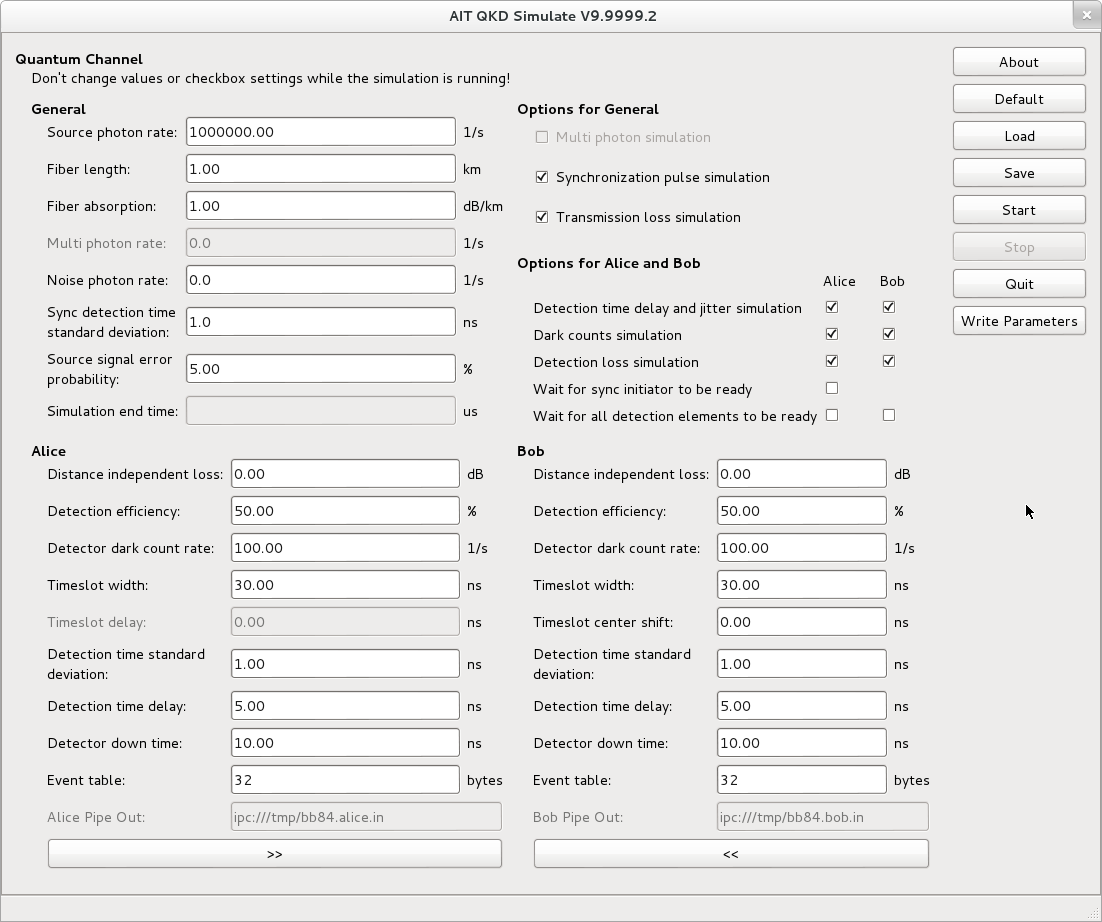
\includegraphics[angle=90,width=\textwidth,keepaspectratio]{images/gui.png}
\caption{The graphical user interface}
\label{fig:gui}
\end{figure}

\refstepcounter{footnote}
\newcounter{fnmodinfo}
\setcounter{fnmodinfo}{\value{footnote}}

\subsection{General Inputs}
\label{subsec:gui_general}

\subsubsection{Source photon rate}
The rate at which photon pairs are generated by \textbf{source}. Photon pair generation is assumed to be a Poisson process so that the time between each pair of consecutive photon generation events has an exponential distribution.

Modifying this input parameter effects a change of the following properties\hyperlink{fn:modinfo}{\footnotemark[\value{fnmodinfo}]}:\\
\texttt{m\_cChannel->m\_cSource.m\_nPhotonRate}

\footnotetext[\value{fnmodinfo}]{\hypertarget{fn:modinfo}A change of the listed properties may also cause further changes of other properties in consequence - refer to the descriptions of the specific components in section \ref{sec:comp} for further information.}

\subsubsection{Fiber length}
The length of the quantum transmission fiber and the sync pulse transmission fiber. Note that the length parameter is only used to simulate transmission loss according to the specified fiber absorption (see subsection \ref{subsubsec:gui_general_fiber_absorption}) in case that the ``Transmission loss simulation'' checkbox has been checked (see subsection \ref{subsubsec:gui_general_options_transmission_loss_simulation}), but no fiber delay is simulated, because ignoring it does not essentially change the simulation behaviour (except for a time shift) but helps to speed up the simulation and to reduce the simulators memory usage.

Modifying this input parameter effects a change of the following properties\hyperlink{fn:modinfo}{\footnotemark[\value{fnmodinfo}]}:\\
\texttt{m\_cChannel->m\_cFiber.m\_nLength}

\subsubsection{Fiber absorption}
\label{subsubsec:gui_general_fiber_absorption}
The quantum transmission fiber's absorption coefficient. Note that the sync pulse transmission fiber is assumed to be lossless.

Modifying this input parameter effects a change of the following properties\hyperlink{fn:modinfo}{\footnotemark[\value{fnmodinfo}]}:\\
\texttt{m\_cChannel->m\_cFiber.m\_nAbsorptionCoefficient}

\subsubsection{Noise photon rate}
The rate of noise photons generated by the \textbf{noise photon source} located inside \textbf{fiber}. It is assumed that noise photon generation is a Poisson process and that the generated noise photons are non-polarised.

Modifying this input parameter effects a change of the following properties\hyperlink{fn:modinfo}{\footnotemark[\value{fnmodinfo}]}:\\
\texttt{m\_cChannel->m\_cFiber.m\_noise\_photon\_source.m\_noise\_photon\_rate}

\subsubsection{Sync detection time standard deviation}
The jitter assigned to the \textbf{sync pulse receiver} for sync pulse detection. A Gaussian distribution of the jitter is assumed, except for a cutoff at minus five standard deviations (refer to sections \ref{subsec:comp_channel} and \ref{par:comp_detector_syncprcv} for further information on the influence of this parameter).

Modifying this input parameter effects a change of the following properties\hyperlink{fn:modinfo}{\footnotemark[\value{fnmodinfo}]}:\\
\texttt{m\_cChannel->m\_nStndSyncDeviation}

\subsubsection{Source signal error probability}
Whenever the \textbf{source} generates an entangled photon pair, the \texttt{entanglement\_error} property of the generated \texttt{photon\_pair} object (see section \ref{subsec:concepts_photons}) is set according to the value specified for the source signal error probability.

Modifying this input parameter effects a change of the following properties\hyperlink{fn:modinfo}{\footnotemark[\value{fnmodinfo}]}:\\
\texttt{m\_cChannel->m\_cSource.m\_nSignalErrorProbablity}

\subsubsection{Simulation end time}
The time until which the simulation (starting from time 0) should run. This value is only used in \textit{free running mode}.

Modifying this input parameter effects a change of the following properties\hyperlink{fn:modinfo}{\footnotemark[\value{fnmodinfo}]}:\\
\texttt{m\_cChannel->m\_ch\_event\_manager.m\_sim\_end\_time}

\subsection{General Options}
\label{subsec:gui_general_options}

\subsubsection{Synchronization pulse simulation}
\label{subsubsec:gui_general_syncpulse}
If this checkbox is checked, the \textit{sync mode} or one of its variants (depending on the settings described in subsections \ref{subsubsec:gui_abopt_wait_for_sync_initiator} and \ref{subsubsec:gui_abopt_wait_for_all}) is used. If it is not checked, \textbf{detector alice} and \textbf{detector bob} are set in \textit{free running mode}.

Changing this option effects a change of the following properties\hyperlink{fn:modinfo}{\footnotemark[\value{fnmodinfo}]}:\\
\texttt{m\_cChannel->m\_cDetectorAlice->m\_detection\_mode}\\
\texttt{m\_cChannel->m\_cDetectorBob->m\_detection\_mode}

\subsubsection{Transmission loss simulation}
\label{subsubsec:gui_general_options_transmission_loss_simulation}
If this checkbox is checked, the fiber absorption coefficient as described in subsection \ref{subsubsec:gui_general_fiber_absorption} is assigned to the quantum transmission fiber. If it is not checked, the quantum transmission fiber is simulated to be lossless.

Changing this option effects a change of the following properties\hyperlink{fn:modinfo}{\footnotemark[\value{fnmodinfo}]}:\\
\texttt{m\_cChannel->m\_cFiber.m\_bLoss}

\subsection{Alice Inputs}
\label{subsec:gui_alice}

\subsubsection{Distance independent loss}
A distance independent loss assigned to the \textbf{detector optics} of \textbf{detector alice}.

Modifying this input parameter effects a change of the following properties\hyperlink{fn:modinfo}{\footnotemark[\value{fnmodinfo}]}:\\
\texttt{m\_cChannel->m\_cDetectorAlice.m\_nLossRate}

\subsubsection{Detection efficiency}
A detection efficiency assigned to the \textbf{detector optics} of \textbf{detector alice}.

Modifying this input parameter effects a change of the following properties\hyperlink{fn:modinfo}{\footnotemark[\value{fnmodinfo}]}:\\
\texttt{m\_cChannel->m\_cDetectorAlice.m\_nEfficiency}

\subsubsection{Detector dark count rate}
The dark count rate for \textbf{detector alice}. This detector dark count rate is assigned as dark count rate parameter to each of the four \textbf{detection element}s. Dark counts for all detection elements are assumed to be Poisson processes, but they can only occur if the specific detection element is enabled and ready (not in down state).

Modifying this input parameter effects a change of the following properties\hyperlink{fn:modinfo}{\footnotemark[\value{fnmodinfo}]}:\\
\texttt{m\_cChannel->m\_cDetectorAlice.m\_nDarkCountRate}

\subsubsection{Timeslot width}
The duration of the window produced by the \textbf{window generator}.

Modifying this input parameter effects a change of the following properties\hyperlink{fn:modinfo}{\footnotemark[\value{fnmodinfo}]}:\\
\texttt{m\_cChannel->m\_cDetectorAlice.m\_nTimeSlotWidth}

\subsubsection{Detection time standard deviation}
\label{subsubsec:gui_alice_det_time_stnd_dev}
The jitter of photon detection set for the four \textbf{detection element}s. A Gaussian distribution of jitter is assumed.

Modifying this input parameter effects a change of the following properties\hyperlink{fn:modinfo}{\footnotemark[\value{fnmodinfo}]}:\\
\texttt{m\_cChannel->m\_cDetectorAlice.m\_nPhotonTimeStndDeviation}

\subsubsection{Detection time delay}
\label{subsubsec:gui_alice_det_time_delay}
The delay of photon detection set for the four \textbf{detection element}s. Note that this parameter should always be set to a value greater or equal than at least three times the detection time standard deviation (see subsection \ref{subsubsec:gui_alice_det_time_stnd_dev}), because acausal detection times are not allowed in the simulation and if they would occur, the random variable for the jitter time is ``reshuffled'' until a causal detection time (sum of delay time plus jitter time) is obtained. This effectively causes the originally Gaussian probability distribution of detection times to be cut off at zero and therefore a distortion to a non-Gaussian distribution. This effect rarely occurs, however, if the detection time delay is set to at least three times the detection time standard deviation, as recommended.

Modifying this input parameter effects a change of the following properties\hyperlink{fn:modinfo}{\footnotemark[\value{fnmodinfo}]}:\\
\texttt{m\_cChannel->m\_cDetectorAlice.m\_nPhotonTimeDelay}

\subsubsection{Detector down time}
The down time configured for the \textbf{detection element}s.

Modifying this input parameter effects a change of the following properties\hyperlink{fn:modinfo}{\footnotemark[\value{fnmodinfo}]}:\\
\texttt{m\_cChannel->m\_cDetectorAlice.m\_nDownTime}

\subsubsection{Event table}
The size of the \textbf{event buffer}'s key buffer in bytes. Each byte can store the contents of the event latch for two sync pulses (for the first sync pulse, the upper half byte is filled, and for the second sync pulse the lower half byte is filled). The bit ordering used for the four detection elements is (from high to low bit): M P V H (minus, plus, vertical, horizontal). 

Modifying this input parameter effects a change of the following properties\hyperlink{fn:modinfo}{\footnotemark[\value{fnmodinfo}]}:\\
\texttt{m\_cChannel->m\_cDetectorAlice.m\_nEventTableSize}

\subsection{Bob Inputs}

The inputs for Bob are almost the same as for Alice, therefore only the differences to Alice's side are explained.

\subsubsection{Timeslot center shift}
This parameter specifies the mean time shift between the center of the window generated by Bob's \textbf{window generator} and the associated photon coming to \textbf{detector bob}. A positive value specifies that the photon comes later than the center of the window, a negative value specifies that the photon comes earlier.

Modifying this input parameter effects a change of the following properties\hyperlink{fn:modinfo}{\footnotemark[\value{fnmodinfo}]}:\\
\texttt{m\_cChannel->m\_timeslot\_center\_shift}

\subsection{Options for Alice and Bob}
\label{subsec:gui_abopt}

\subsubsection{Detection time delay and jitter simulation}
If this checkbox is checked, delay and jitter times are simulated for the \textbf{detection element}s. If it is unchecked, the delay and jitter times for the \textbf{detection element}s are set to zero.

Changing these options effects a change of the following properties (for Alice or Bob, respectively)\hyperlink{fn:modinfo}{\footnotemark[\value{fnmodinfo}]}:\\
\texttt{m\_cChannel->m\_cDetectorAlice->m\_bJitter}\\
\texttt{m\_cChannel->m\_cDetectorBob->m\_bJitter}

\subsubsection{Dark counts simulation}
If this checkbox is checked, dark counts are simulated for the \textbf{detection element}s. If it is unchecked, the dark count rate of the \textbf{detection element}s is set to zero.

Changing these options effects a change of the following properties (for Alice or Bob, respectively)\hyperlink{fn:modinfo}{\footnotemark[\value{fnmodinfo}]}:\\
\texttt{m\_cChannel->m\_cDetectorAlice->m\_bDarkCounts}\\
\texttt{m\_cChannel->m\_cDetectorBob->m\_bDarkCounts}

\subsubsection{Detection loss simulation}
If this checkbox is checked, the distance independent loss, detection efficiency and detector down time parameters are assigned to the specific detector. If this checkbox is not checked, the detector is simulated to be lossless and to have zero down time.

Changing these options effects a change of the following properties (for Alice or Bob, respectively)\hyperlink{fn:modinfo}{\footnotemark[\value{fnmodinfo}]}:\\
\texttt{m\_cChannel->m\_cDetectorAlice->m\_bLoss}\\
\texttt{m\_cChannel->m\_cDetectorBob->m\_bLoss}

\subsubsection{Wait for sync initiator to be ready}
\label{subsubsec:gui_abopt_wait_for_sync_initiator}
If this checkbox is checked and the ``Wait for all detectors to be ready'' for Alice is not checked, \textbf{detector alice} is set into \textit{sync mode - wait for sync initiator to be ready}. If this checkbox is not checked (or not available (for Bob's side), respectively) and the ``Wait for all detectors to be ready'' checkbox is also unchecked but the ``Synchronization pulse simulation'' checkbox is checked (see section \ref{subsubsec:gui_general_syncpulse}), the specific \textbf{detector} is set into \textit{sync mode}.

Changing this option effects a change of the following properties\hyperlink{fn:modinfo}{\footnotemark[\value{fnmodinfo}]}:\\
\texttt{m\_cChannel->m\_cDetectorAlice->detection\_mode}

\subsubsection{Wait for all detection elements to be ready}
\label{subsubsec:gui_abopt_wait_for_all}
If this checkbox is checked, the specific detector is set into \textit{sync mode - wait for all detection elements to be ready}. If this checkbox is not checked and the ``Wait for sync initiator to be ready'' checkbox is also not checked (or not available (for Bob's side), respectively) but the ``Synchronization pulse simulation'' checkbox is checked (see section \ref{subsubsec:gui_general_syncpulse}), the specific \textbf{detector} is set into \textit{sync mode}.

Changing these options effects a change of the following properties (for Alice or Bob, respectively)\hyperlink{fn:modinfo}{\footnotemark[\value{fnmodinfo}]}:\\
\texttt{m\_cChannel->m\_cDetectorAlice->detection\_mode}\\
\texttt{m\_cChannel->m\_cDetectorBob->detection\_mode}

\subsection{Click Buttons}

\subsubsection{About}
Displays the ``About'' dialog box.

\subsubsection{Default}
Loads the default values for the parameters, which are defined in \texttt{default\_values.cpp}.

\subsubsection{Load}
Opens a dialog box that allows to select a configuration file from which parameters should be loaded.

\subsubsection{Save}
Open a dialog box that allows to save the configured parameters to a configuration file. Note that checkbox settings are not stored in the configuration file.

\subsubsection{Start}
Start the quantum channel simulation.

\subsubsection{Stop}
Terminate the quantum channel simulation.

\subsubsection{Quit}
Terminate the QKD-Simulate program.

\newpage
\begin{thebibliography}{9}
\addcontentsline{toc}{section}{References}

\bibitem{daSilva2011}
  Thiago Ferreira da Silva, Guilherme B. Xavier, and Jean Pierre von der Weid,
  ``Real-time Characterization of Gated-Mode Single-Photon Detectors'',
  IEEE J. Quantum Electron. 47, 1251-1256,
  2011.
  DOI: 10.1109/JQE.2011.2163622

\end{thebibliography}

\newpage
\appendix
\addcontentsline{toc}{section}{Appendices}

\section{Extension of the QKD Simulator's Functionality}

The framework provided by the event and photon pair management in the QKD simulator can be used to extend its functionality by changing the implementation of some system components or adding new ones. Here are some important remarks for doing so:

\begin{itemize}

\item If a new system component is to be created, it must be implemented in a class that is derived from the \texttt{ch\_event\_handler} base class defined in \texttt{channel/ch\_event\_handler.h} and \texttt{channel/ch\_event\_handler.cpp}. Especially, the new component should redefine the virtual \texttt{handle\_event} function that defines the component's behaviour during the simulation by specifying how it reacts to specific events.

\item If a channel event handler contains subcomponents, it should redefine the \texttt{init\_evh} function originally defined in the \texttt{ch\_event\_handler} base class, and the redefined function should always at first call the base class function by executing the line:
\begin{lstlisting}
this->ch_event_handler::init_evh(evh_parent, evm, phpm);
\end{lstlisting}
and secondly, for all subcomponents, it should call their \texttt{init\_evh} function by executing:
\begin{lstlisting}
subcomponentname.init_evh(this, evm, phpm);
\end{lstlisting}
where \texttt{subcomponentname} is to be replaced by the name of the specific subcomponent.

\item All channel event handlers can use the following pointers contained in the \texttt{ch\_event\_handler} base class:

\begin{itemize}

\item \texttt{m\_evh\_parent} is a pointer to the parent event handler (or \texttt{nullptr} if no parent is existing).

\item \texttt{m\_evm} is a pointer to the channel event manager.

\item \texttt{m\_phpm} is a pointer to the photon pair manager.

\end{itemize}

\item If a component should create new events during the simulation, refer to section \ref{subsec:concepts_events} where the rules for newly created events and component interaction are described. Especially, it should be kept in mind that no acausal events may be created (which means that the \texttt{m\_time} member of the newly created \texttt{ch\_event} must not be set to a value smaller than \texttt{m\_evm->get\_time()} (this function call returns the current simulation time)).

\item If a component needs to create or process photon pairs, refer to section \ref{subsec:concepts_photons} where the rules for photon pair creation and handling are described. Especially, it should be kept in mind that for each created \texttt{photon\_pair} object, it must be ensured that there is a channel event handler that deletes the \texttt{photon\_pair} object at the end of its usage time, because the photon pair manager does not by itself automatically delete \texttt{photon\_pair} objects.

\item The \texttt{ch\_event\_manager} provides a \texttt{remove\_event} function that allows to remove an event by specifying its event ID, so that it will not be handled. However, this function should be used with care, because it has some limitations. Especially, when an event is created and afterwards removed by this function, this causes a temporal ``memory leak'' of at least 20 to 24 Byte size (or maybe some more due to overhead hidden in the internal implementations of the STL containers used by the QKD simulator) that persists until the simulation reaches the time when the originally created event would have occurred if it had not been removed. So, calling this function extremely often, especially for events that lie in far future, could in the worst case cause the main memory to be used up. In order to avoid this adverse effect, it will be necessary to change the implementation of the \texttt{ch\_event\_manager}. In particular, it seems to be necessary to write a new, more flexible implementation of a priority queue (or using a library that provides such a container) instead of using the STL library's \texttt{priority\_queue} container which regrettably doesn't seem to support random element removal.

\end{itemize}

\subsection{Adding Afterpulsing Simulation to the Detection Elements}
\label{subsec:after_pulsing}

\subsubsection{Derivation of the Afterpulsing Probability Distribution Function}

In this section, a theoretical derivation of the afterpulse probability distribution function for the detection elements will be provided, and it will be described how this distribution function can be used as a basis for adding afterpulse simulation to the detection element's implementation.\\
\\
In the following derivations, a single detection element will be treated, and only the time horizon after the last down period (that followed a previous detector pulse) during which no further dark count or incident photon occurs will be considered.  

Let $F_1(t)$ denote the probability that the first afterpulse occurs in the time interval $[0, t]$, where the time point $t = 0$ should be the end of the down period after the last detector pulse.

For a very small time difference $\Delta t$, the probability that the first afterpulse occurs in the time interval $(t, t + \Delta t]$ is assumed to be given as
\begin{equation}
\label{eq:f1start}
F_1(t+\Delta t)-F_1(t)=(1-F_1(t)) \cdot c \cdot \mathrm{exp}(-t/\tau)\,\Delta t
\end{equation}
where $(1-F_1(t))$ is the probability that the first afterpulse did not occur in the time interval $[0, t]$ and $c \cdot \mathrm{exp}(-t/\tau)$ is an afterpulse ``rate'' that is assumed to be proportional to the number of trapped carriers, which in turn is assumed to decay exponentially with a detrapping lifetime $\tau$ (cf. \cite[p.~2]{daSilva2011}). The product $c \cdot \mathrm{exp}(-t/\tau)\,\Delta t$ is therefore the probability that an afterpulse occurs in the time interval $(t, t + \Delta t]$ on the condition that no afterpulse occurred during the time interval $[0, t]$. The constant $c$ is proportional to the number of initially filled traps and will be determined later.

Dividing both sides of Equation \ref{eq:f1start} by $\Delta t$, performing the limit $\Delta t \to 0$ and using
\begin{equation}
\label{eq:f1dlim}
F_1'(t)=\lim_{\Delta t \to 0} \frac{F_1(t+\Delta t) - F_1(t)}{\Delta t}
\end{equation}
(where the limit is assumed to exist because Equation \ref{eq:f1start} should hold asymptotically for $\Delta t$ approaching zero) leads to the differential equation
\begin{equation}
\label{eq:f1de}
F_1'(t)=(1-F_1(t)) \cdot c \cdot \mathrm{exp}(-t/\tau)
\end{equation}
Solving this for $F_1(t)$ and applying the initial condition $F_1(0)=0$ gives the result
\begin{equation}
\label{eq:f1sol}
F_1(t)=1-\mathrm{exp}(-c \tau (1 - \mathrm{exp}(-t/\tau)))
\end{equation}
If it is now assumed that the detection element's dark count rate and the incident photon rate are so small that the average time between dark count or incident photon events is much greater than $\tau$, the total afterpulse probability is obtained from Equation \ref{eq:f1sol} as
\begin{equation}
\label{eq:ptotal}
p_{total}=\lim_{t \to \infty} F_1(t)=1-\mathrm{exp}(-c \tau)
\end{equation}
because this is just the probability that the first afterpulse occurs in the time interval $[0, \infty)$, which means it is the probability that any afterpulse occurs at all. This result shows that $p_{total}$ is always strictly smaller than one. As mentioned above, Equation \ref{eq:ptotal} is only valid in the case that dark counts or incident photons are coming only very seldom during a time period in the order of magnitude of $\tau$, because if the are coming more frequently, the probability that a dark count or incident photon occurs before a possible afterpulse could occur becomes significant.

Solving Equation \ref{eq:ptotal} for $c$ gives
\begin{equation}
\label{eq:csol}
c=-\frac{1}{\tau}\mathrm{ln}(1-p_{total})
\end{equation}

\subsubsection{Simulation Method for Afterpulsing}

The results of the previous subsection can now be used to simulate afterpulsing by application of the inverse transformation method. For this method, the inverse function of $F_1(t)$ is needed, which will be denoted as $F_1^{-1}(u)$ and is obtained by solving
\begin{equation*}
u=F_1(t)
\end{equation*}
for $t = F_1^{-1}(u)$ using Equation \ref{eq:f1sol}, which leads to
\begin{equation}
\label{eq:f1inv}
F_1^{-1}(u)=-\tau\,\mathrm{ln}\left(1+\frac{\mathrm{ln}(1-u)}{c\tau}\right)
\end{equation}

The simulation algorithm now works as follows:

\begin{enumerate}

\item Obtain the parameters $\tau$ and $p_{total}$ from data sheets or measurements of the detection element.

\item Calculate $c$ from Equation \ref{eq:csol}

\item Generate a random number $u$ that is uniformly distributed in the interval $[0, 1)$.

\item If $u \geq p_{total}$, no afterpulse shall be generated. However, if $u < p_{total}$, calculate $t$ using Equation~\ref{eq:f1inv} as
\begin{equation*}
t=F_1^{-1}(u)
\end{equation*}
and create an afterpulse event that occurs at time $t$ (measured relative to the end of the previous down period).

\end{enumerate}

The procedure described above is not complete, however, because it does not yet cover the cases that a dark count or incident photon event occurs before a previously set afterpulse event is handled, or the case that the detection element is disabled after an afterpulse event has been set. Therefore, the procedure described above is just to be seen as a basis that must be extended by additional functionality so that it can be used in the detection elements.


\end{document}
